\documentclass[a4paper, 12pt]{article}
\usepackage{graphicx}
\usepackage[czech]{babel}
\usepackage[utf8]{inputenc}
\usepackage[T1]{fontenc}
\usepackage{amsmath}
\usepackage{amssymb}
\usepackage{pdfpages}
\usepackage{mathrsfs}
\usepackage{siunitx}
\usepackage{xcolor}
\usepackage{titlesec}
\usepackage{wrapfig}

\setcounter{secnumdepth}{4}

\titleformat{\paragraph}
{\normalfont\normalsize\bfseries}{\theparagraph}{1em}{}
\titlespacing*{\paragraph}
{0pt}{3.25ex plus 1ex minus .2ex}{1.5ex plus .2ex}

\sisetup{%
     output-decimal-marker = {.},
     inter-unit-product = \ensuremath{{}\cdot{}}
        }
        
\author{A18B0474P - Jiří Švamberg}
\title{Projekt 5}
\date{\today}

\setlength{\hoffset}{-1.8cm} 
\setlength{\voffset}{-2cm}
\setlength{\textheight}{24.0cm} 
\setlength{\textwidth}{17cm}

\begin{document}
	\begin{titlepage}
		\maketitle
		\begin{figure}
			\centering
			
\includegraphics{Obrazky/FAV-logo.pdf}
			
\includegraphics{Obrazky/zcu-logo.pdf}
			
\includegraphics[scale=0.3]{Obrazky/KKY_logo_cz.pdf}
		\end{figure}
		\thispagestyle{empty}
		\newpage
	\end{titlepage}

	\tableofcontents
	\newpage
	\section{Zadání}
		\begin{enumerate}
			\item Navrhněte zjednodušený model soustavy kvadrotorová helikoptéra - břemeno\\
			\item Pro zjednodušený model navrhněte regulátor\\
			\item Implementujte regulátor do zjednodušeného modelu\\
		\end{enumerate}
		\clearpage
	\section{Zjednodušený model}
		\subsection{Návrh zjednodušeného modelu}		
			Zjednodušený model budeme navrhovat ve 2D jako kyvadlo zavěšené na vozíku.
			\begin{wrapfigure}{r}{0pt}
				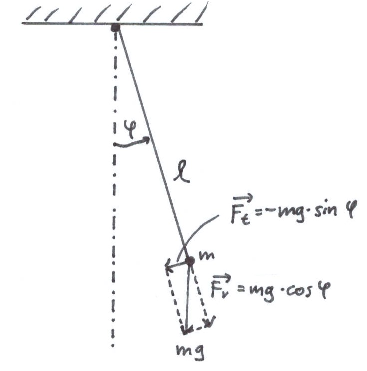
\includegraphics[scale=0.75]{Obrazky/Kyvadlo.pdf}
				\caption{Schéma jednoduchého kyvadla}
				\label{schema kyvadla}
			%\end{wrapfigure}
			%\begin{wrapfigure}{r}{0pt}
				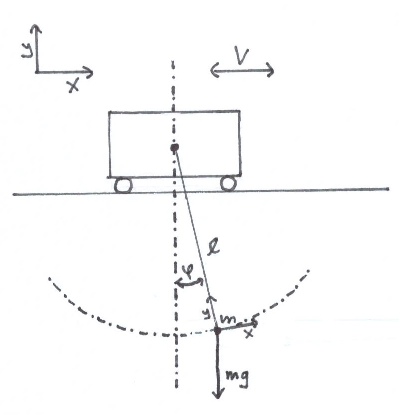
\includegraphics[scale=0.75]{Obrazky/Vozik-kyvadlo.pdf}
				\caption{Schéma soustavy vozík-kyvadlo}
				\label{schema vozik-kyvadlo}
			\end{wrapfigure}
			Pro potřeby návrhu tohoto modelu budeme uvažovat lano závěsu jako dokonale nepružné, o stálé délce $l$ a nulové hmotnosti $m_l = \SI{0}{\kilogram}$. Úhel vychýlení závěsu od osy vozíku označíme jako $\varphi$. Jako těleso si představíme bezrozměrný hmotný bod o hmotnosti $m$.\\
			Pro jednoduché kyvadlo připevněné k nepohybujícímu se tělesu o kinetické energii $T = \frac{1}{2}mv^2$ a potenciální energii $V = -mgl\cos\varphi$ (obr. \ref{schema kyvadla}) platí pohybová rovnice:
			\begin{align*}
				\ddot{\varphi}+\frac{g}{l}\sin\varphi=0
			\end{align*}
			Po zavěšení jednoduchého kyvadla na vozík(obr. \ref{schema vozik-kyvadlo}) budeme muset ještě do modelu přidat dynamiku vozíku o hmotnosti $M$. Na ten může působit síla ve směru osy x. Pro hmotný bod, zavěšený na laně budeme muset spočítat souřadnice $\left[u, v\right]$, jelikož při pohybu vozíku se nepohybuje po jasné trajektorii (kružnice, přímka):
			\begin{align*}
				u &= x + l\sin\varphi \rightarrow \dot{u} = \dot{x}+l\dot{\varphi}\cos\varphi\\
				v &= -l\cos\varphi \rightarrow \dot{v} = l\dot{\varphi}\sin\varphi
			\end{align*} 
			K odvození modelu využijeme Lagrangeovu metodu.\\
			Potenciální energii $V$ budeme uvažovat stejnou, jako u jednoduchého kyvadla.
			\begin{align*}
				V = -mgl\cos{\varphi}
			\end{align*}
			Jako základ pro vzorec kinetické energie použijeme vzorec kinetické energie obyčejného matematického kyvadla $T = \frac{1}{2}mv^2$. Musíme ale uvažovat rychlost ve směru všech souřadnic ($x$, $u$, $v$).
			\begin{align*}
				T &= \frac{1}{2}M\dot{x}^2+\frac{1}{2}m\dot{u}^2+\frac{1}{2}m\dot{v}^2
			\end{align*}
			Po dosazení souřadnic pro hmotný bod zavěšený na laně dostaneme kinetickou energii ve tvaru:
			\begin{align*}
				T &= \frac{1}{2}M\dot{x}^2+\frac{1}{2}m(l\dot{\varphi}\cos\varphi+\dot{x})^2+\frac{1}{2}m(l\dot{\varphi}\sin\varphi)^2
			\end{align*}
			Zjistíme si Lagrangián $L = T - V$:
			\begin{align*}
				L = \frac{1}{2}M\dot{x}^2+\frac{1}{2}ml^2\dot{\varphi}^2\cos^2\varphi+m\dot{x}l\dot{\varphi}\cos\varphi+\frac{1}{2}m\dot{x}^2+\frac{1}{2}ml^2\dot{\varphi}^2\sin^2\varphi+mgl\cos\varphi
			\end{align*}
			, který nyní budeme parciálně derivovat.
			\begin{align*}
				\frac{\partial L}{\partial\dot{x}} &= M\dot{x}+ml\dot{\varphi}\cos\varphi+m\dot{x}\\
				\frac{\partial L}{\partial x} &= 0\\
				\frac{\partial L}{\partial \dot{\varphi}} &= ml^2\dot{\varphi}+m\dot{x}l\cos\varphi\\
				\frac{\partial L}{\partial \varphi} &= -m\dot{x}l\dot{\varphi}\sin\varphi-mgl\sin\varphi
			\end{align*}
			Vztahy pro hledané dvě rovnice vypadají následovně:
			\begin{align*}
				\frac{\mathrm{d}}{\mathrm{d}t}\left(\frac{\partial L}{\partial \dot{x}}\right) - \frac{\partial L}{\partial x} = f\\
				\frac{\mathrm{d}}{\mathrm{d}t}\left(\frac{\partial L}{\partial \dot{\varphi}}\right) - \frac{\partial L}{\partial \varphi} = 0
			\end{align*}
			, kde f je síla působící na vozík. Nyní můžeme dopočítat dvě rovnice modelu vozík-kyvadlo.
			\begin{align*}
				M\dot{x}+ml\ddot{\varphi}\cos\varphi-ml\dot{\varphi}^2\sin\varphi+m\ddot{x} = f\\
				ml\left(l\ddot{\varphi}+\ddot{x}\cos\varphi-\dot{x}\sin\varphi+\dot{x}\dot{\varphi}\sin\varphi+g\sin\varphi\right)=0
			\end{align*}
thr			Dále můžeme vyjádřit nejvyšší derivace:
			\begin{align*}
				\ddot{x} &= \frac{-ml\ddot{\varphi}\cos\varphi+ml\dot{\varphi}^2\sin\varphi+f}{M+m}\\
				\ddot{\varphi} &= \frac{\sin\varphi\left(\dot{x}\dot{\varphi}-\dot{\varphi}+g\right)+\ddot{x}\cos\varphi}{l}
			\end{align*}
			Vidíme, že rovnice na sobě závisí. Můžeme je tedy navzájem dosadit.
			\begin{align*}
				\ddot{x} &= \frac{lm\sin\varphi\dot{\varphi}^2-\dot{x}m\cos\varphi\sin\varphi\dot{\varphi}+f+\dot{x}m\cos\varphi\sin\varphi-gm\cos\varphi\sin\varphi}{m\cos^2\varphi+M+m}\\
				\ddot{\varphi} &= \frac{f\cos\varphi-\dot{x}m\sin\varphi+gm\sin\varphi-M\dot{x}\sin\varphi+Mg\sin\varphi+M\dot{\varphi}\dot{x}\sin\varphi+\dot{\varphi}\dot{x}m\sin\varphi}{l\left(m\cos^2\varphi+M+m\right)}\\
				&+ \frac{\dot{\varphi}^2lm\cos\varphi\sin\varphi}{l\left(m\cos^2\varphi+M+m\right)}
			\end{align*}
		\subsection{Stavový popis zjednodušeného modelu}
			Zavedeme si stavové proměnné
			\begin{align*}
				x &= y_1\\
				\varphi &= y_2\\
				\dot{y_1} = \dot{x} &= y_3\\
				\dot{y_2} = \dot{\varphi} &= y_4\\
				f &= u
			\end{align*}
			Stavový popis systému uvažujeme ve tvaru:
			\begin{align*}
				\dot{x} &= \mathbf{A}\vec{x}+\mathbf{B}\vec{u}\\
				y &= \mathbf{C}\vec{x}   %+\mathbf{D}\vec{u}
			\end{align*}
			, kde 
			\begin{align*}
				\mathbf{A} &= \left[\begin{matrix}
					\frac{\partial f_1}{\partial y_1} & \frac{\partial f_1}{\partial y_2} & \frac{\partial f_1}{\partial y_3} & \frac{\partial f_1}{\partial y_4}\\
					\frac{\partial f_2}{\partial y_1} & \frac{\partial f_2}{\partial y_2} & \frac{\partial f_2}{\partial y_3} & \frac{\partial f_2}{\partial y_4}\\
					\frac{\partial f_3}{\partial y_1} & \frac{\partial f_3}{\partial y_2} & \frac{\partial f_3}{\partial y_3} & \frac{\partial f_3}{\partial y_4}\\
					\frac{\partial f_4}{\partial y_1} & \frac{\partial f_4}{\partial y_2} & \frac{\partial f_4}{\partial y_3} & \frac{\partial f_4}{\partial y_4}	
				\end{matrix}\right]\\
				\mathbf{B} &= \left[\begin{matrix}
					\frac{\partial f_1}{\partial u}\\
					\frac{\partial f_2}{\partial u}\\
					\frac{\partial f_3}{\partial u}\\
					\frac{\partial f_4}{\partial u}
				\end{matrix}\right]\\
				\mathbf{C} &= \left[\begin{matrix}
					1 & 0 & 0 & 0\\
					0 & 1 & 0 & 0\\
					0 & 0 & 1 & 0\\
					0 & 0 & 0 & 1
				\end{matrix}\right]
			\end{align*}
			Dosadíme do rovnic a budeme moct derivovat.
			\begin{align*}
				f_1: \dot{y_1} = &y_3\\
				f_2: \dot{y_2} = &y_4\\
				f_3: \dot{y_3} = & \frac{lm\sin(y_2)y_4^2-y_3m\cos(y_2)\sin(y_2)y_4+u+y_3m\cos(y_2)\sin(y_2)-gm\cos(y_2)\sin(y_2)}{m\cos^2(y_2)+M+m}\\
				f_4: \dot{y_4} = &\frac{u\cos(y_2)-y_3m\sin(y_2)+gm\sin(y_2)-My_3\sin(y_2)+Mg\sin(y_2)+My_4y_3\sin(y_2)}{l\left(m\cos^2(y_2)+M+m\right)}\\
				&+ \frac{y_4y_3m\sin(y_2)+y_4^2lm\cos(y_2)\sin(y_2)}{l\left(m\cos^2(y_2)+M+m\right)}
			\end{align*}
			Po zderivování můžeme linearizovat. To chceme udělat okolo rovnovážného bodu, tj. $x = y_1 = 0$, $\varphi = y_2 = \pi$, $\dot{x} = y_3 = 0$ a $\dot{\varphi} = y_4 = 0$, takže tyto hodnoty do vypočítaných hodnot dosadíme a dostaneme tak matice:
			\begin{align*}
				\mathbf{A} &= \left[\begin{matrix}
					0 & 0 & 1 & 0\\
					0 & 0 & 0 & 1\\
					0 & -\frac{gm}{M+2m} & 0 & 0\\
					0 & -\frac{mg+Mg}{l\left(M+2m\right)} & 0 & 0
				\end{matrix}\right]\\
				\mathbf{B} &= \left[\begin{matrix}
					0\\
					0\\
					\frac{1}{M+2m}\\
					-\frac{1}{l\left(M+2m\right)}
				\end{matrix}\right]
			\end{align*}
			Výsledný stavový popis v okolí pracovního bodu $\left[\dot{x}, \dot{\varphi}, x, \varphi\right]=\left[0, 0, 0, 0\right]$ bude tedy vypadat:
			\begin{align*}
				\dot{x}&=\left[\begin{matrix}
					0 & 0 & 1 & 0\\
					0 & 0 & 0 & 1\\
					0 & -\frac{gm}{M+2m} & 0 & 0\\
					0 & \frac{mg+Mg}{l\left(M+2m\right)} & 0 & 0
				\end{matrix}\right]
				\left[\begin{matrix}
					y_1\\
					y_2\\
					y_3\\
					y_4
				\end{matrix}\right]
				+
				\left[\begin{matrix}
					0\\
					0\\
					\frac{1}{M+2m}\\
					-\frac{1}{l\left(M+2m\right)}
				\end{matrix}\right]u\\
				y&=\left[\begin{matrix}
					1 & 0 & 0 & 0\\
					0 & 1 & 0 & 0\\
					0 & 0 & 1 & 0\\
					0 & 0 & 0 & 1
				\end{matrix}\right]
				\left[\begin{matrix}
					y_1\\
					y_2\\
					y_3\\
					y_4
				\end{matrix}\right]
			\end{align*}
		\subsection{Dosazení konkrétních hodnot}
			Nyní si můžeme zvolit konkrétní hodnoty našeho modelu. 
			\begin{align*}
				M &= \SI{15}{\kilo\gram}\\
				m &= \SI{5}{\kilo\gram}\\
				l &= \SI{1}{\meter}\\
				g &= \SI{9,81}{\meter\square\second}\\
			\end{align*}
			Působící sílu můžeme měnit, abychom mohli ověřit chování v různých situacích.
		\clearpage
		\subsection{Grafy}
			\begin{figure}[h]
				\begin{center}
					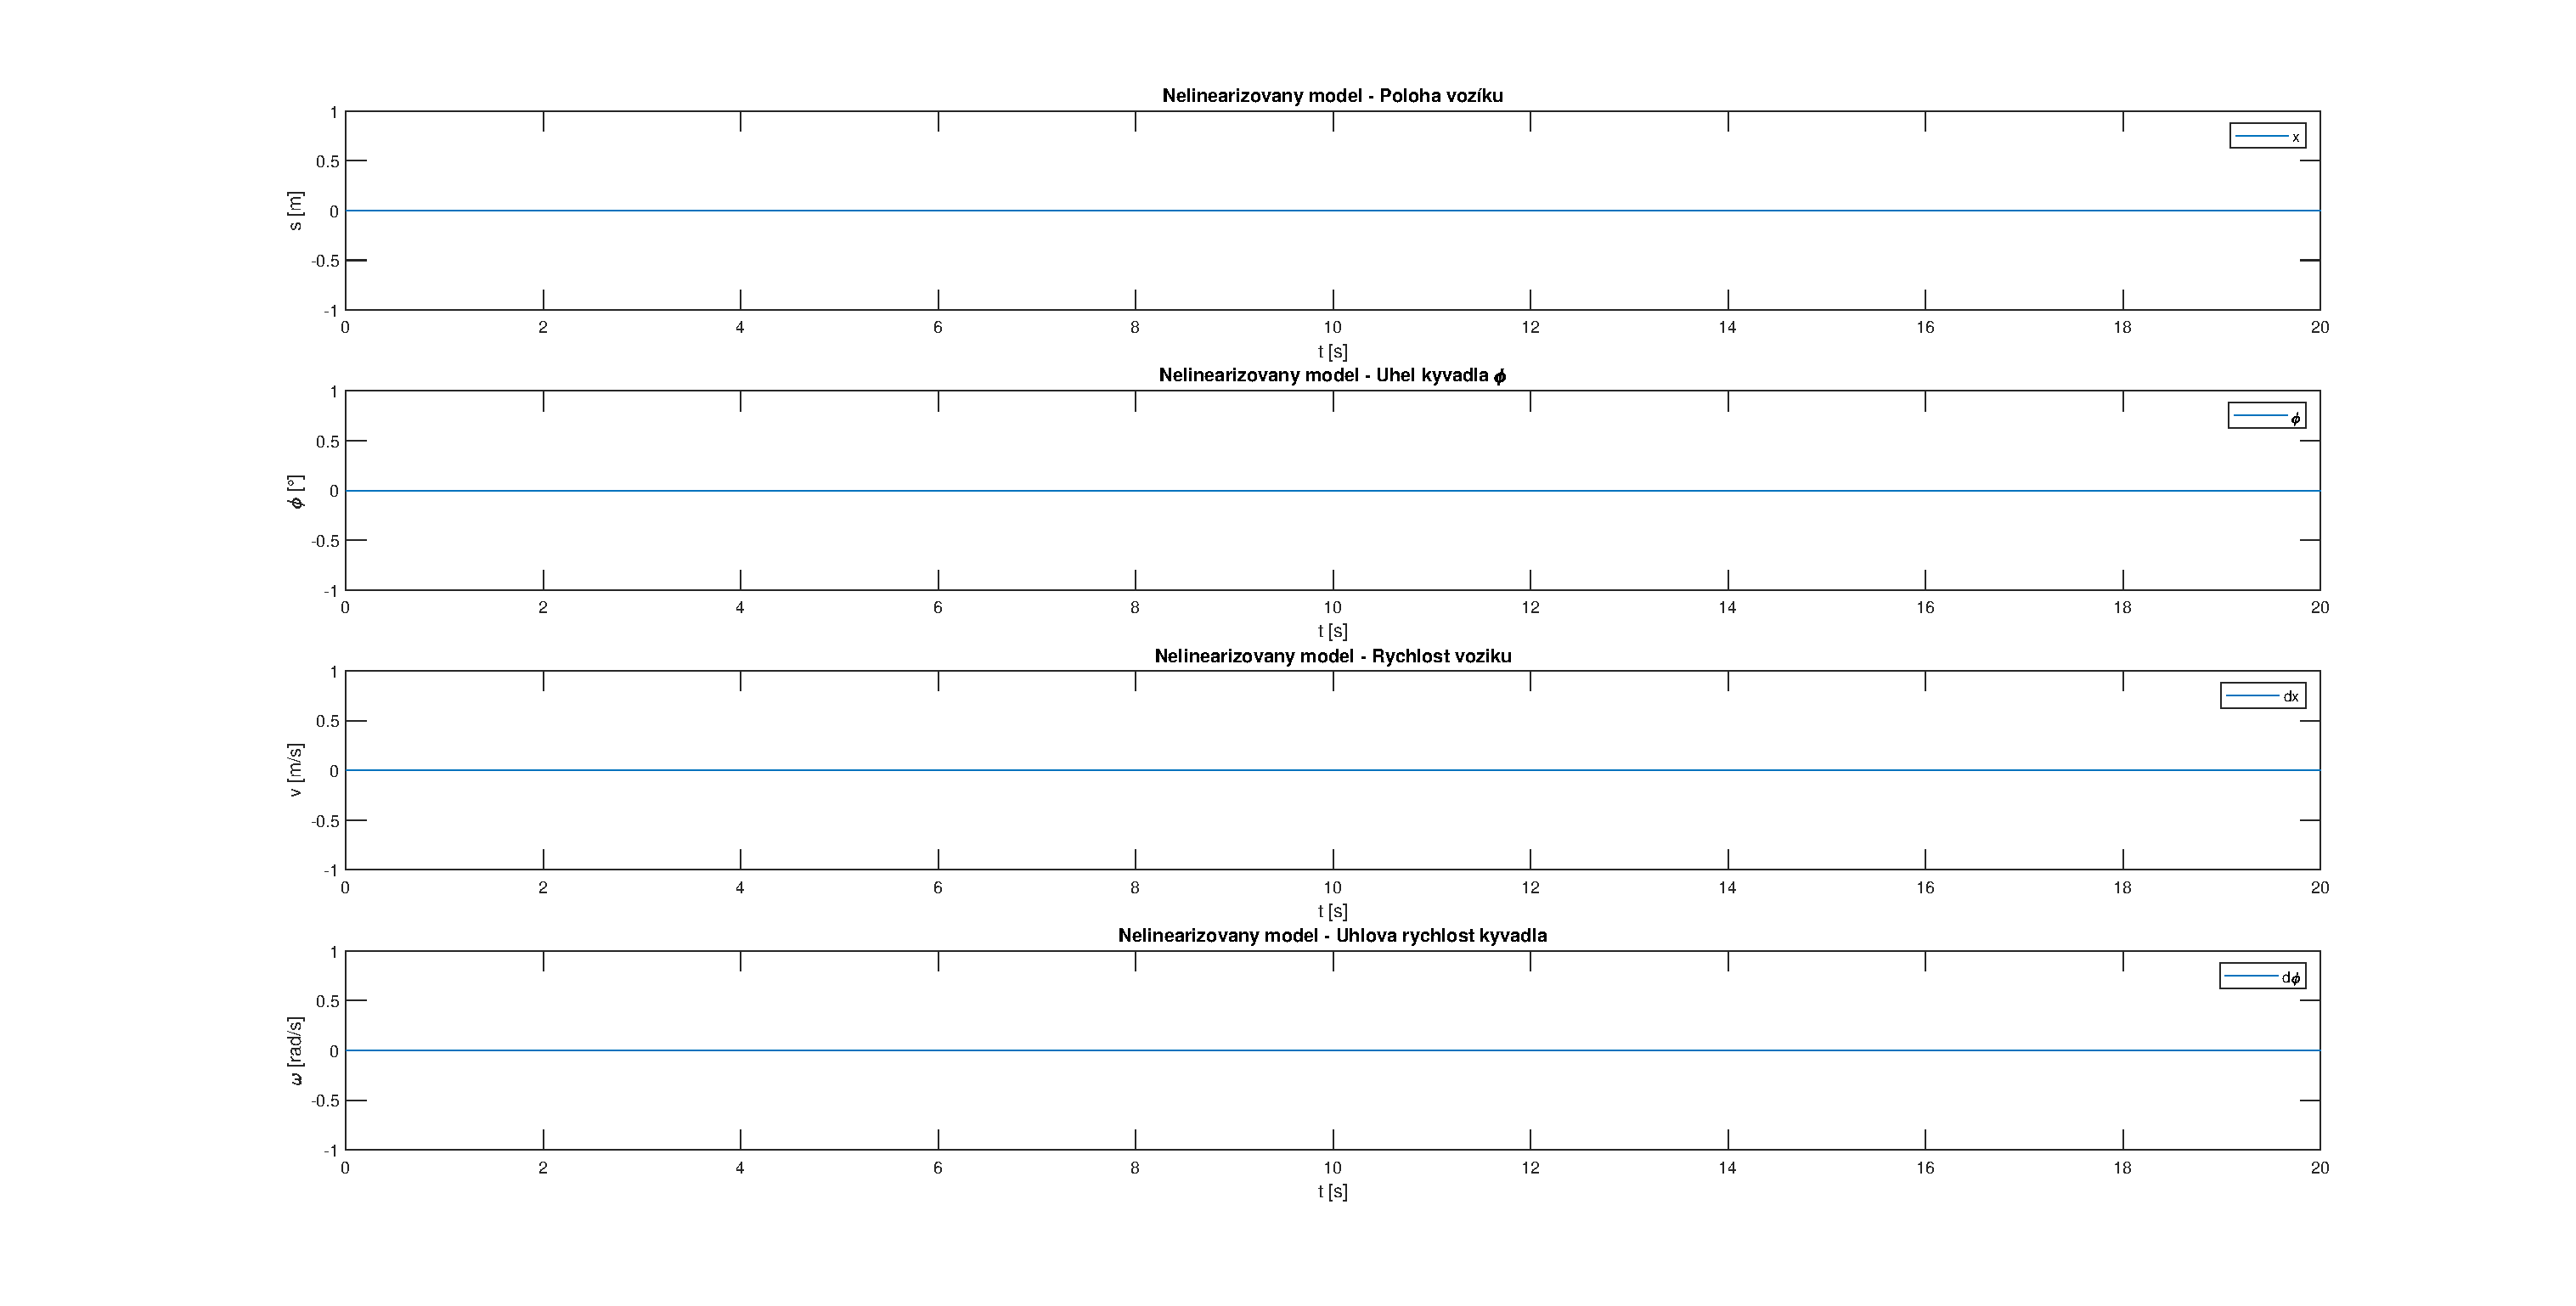
\includegraphics[scale=0.3]{Obrazky/Nel_model_f0_nul.eps}
					\label{Nel_model_f0_nul}
					\caption{Nelineární model při $f=\SI{0}{\newton}$ a nulových p.p.}
				\end{center}
				\begin{center}
					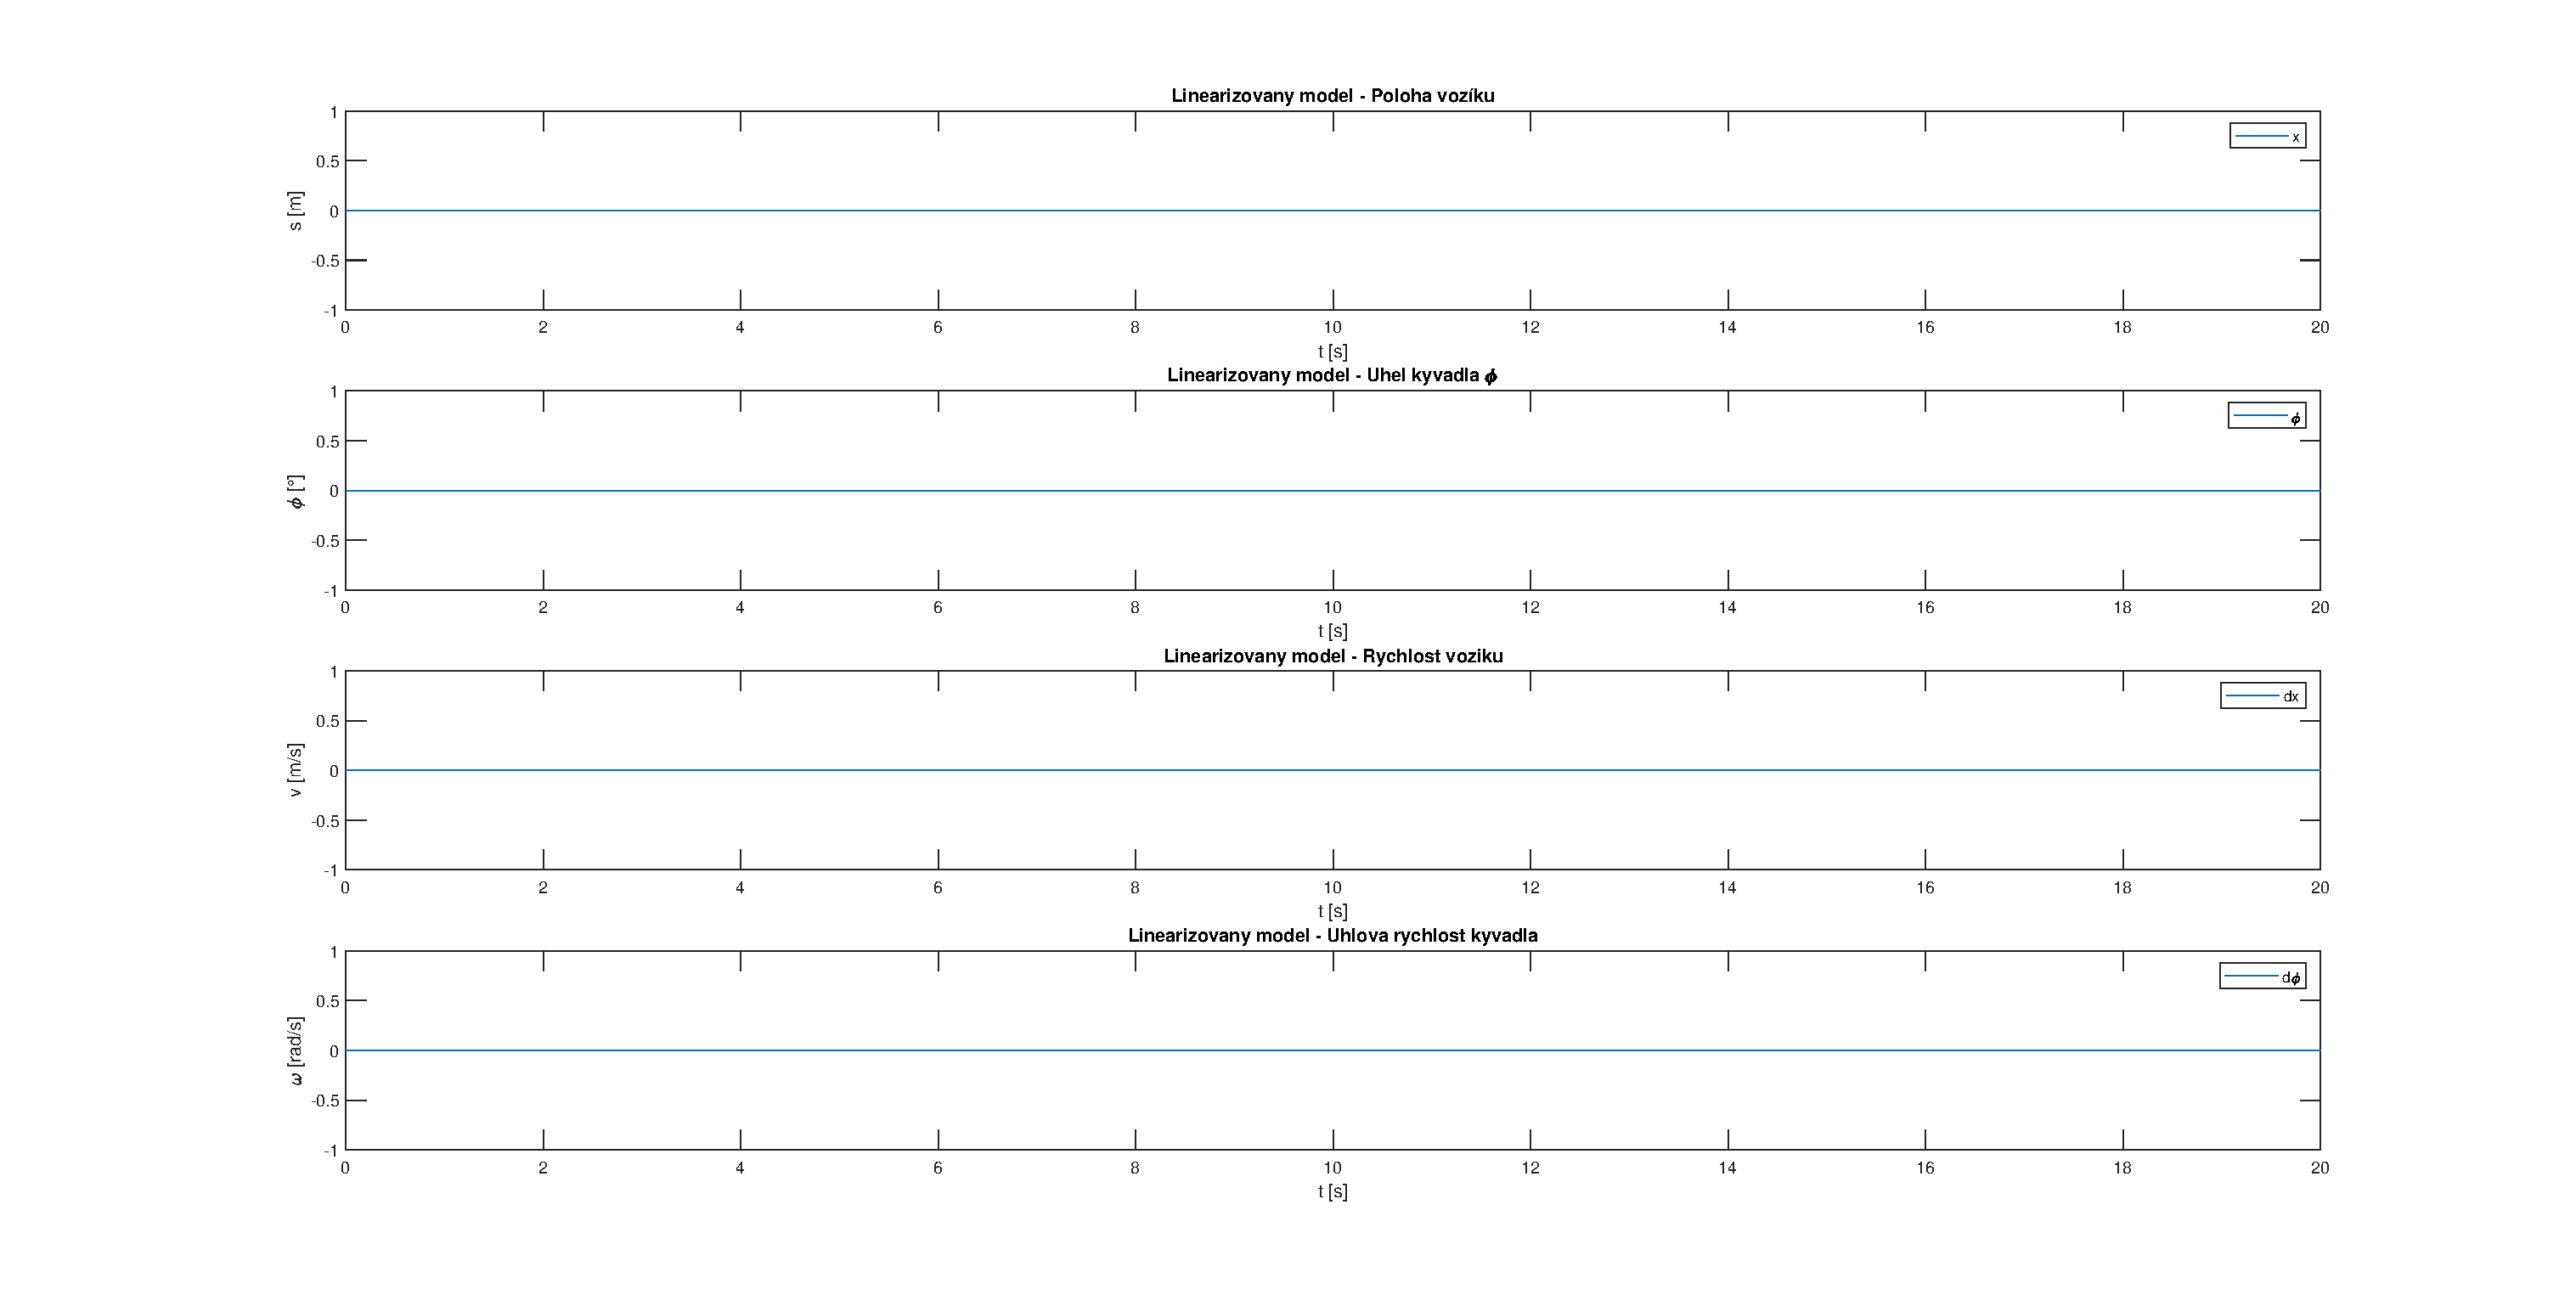
\includegraphics[scale=0.3]{Obrazky/Lin_model_f0_nul.eps}
					\label{Lin_model_f0_nul}
					\caption{Lineární model při $f=\SI{0}{\newton}$ a nulových p.p.}
				\end{center}
			\end{figure}
			\begin{figure}[h]
				\begin{center}
					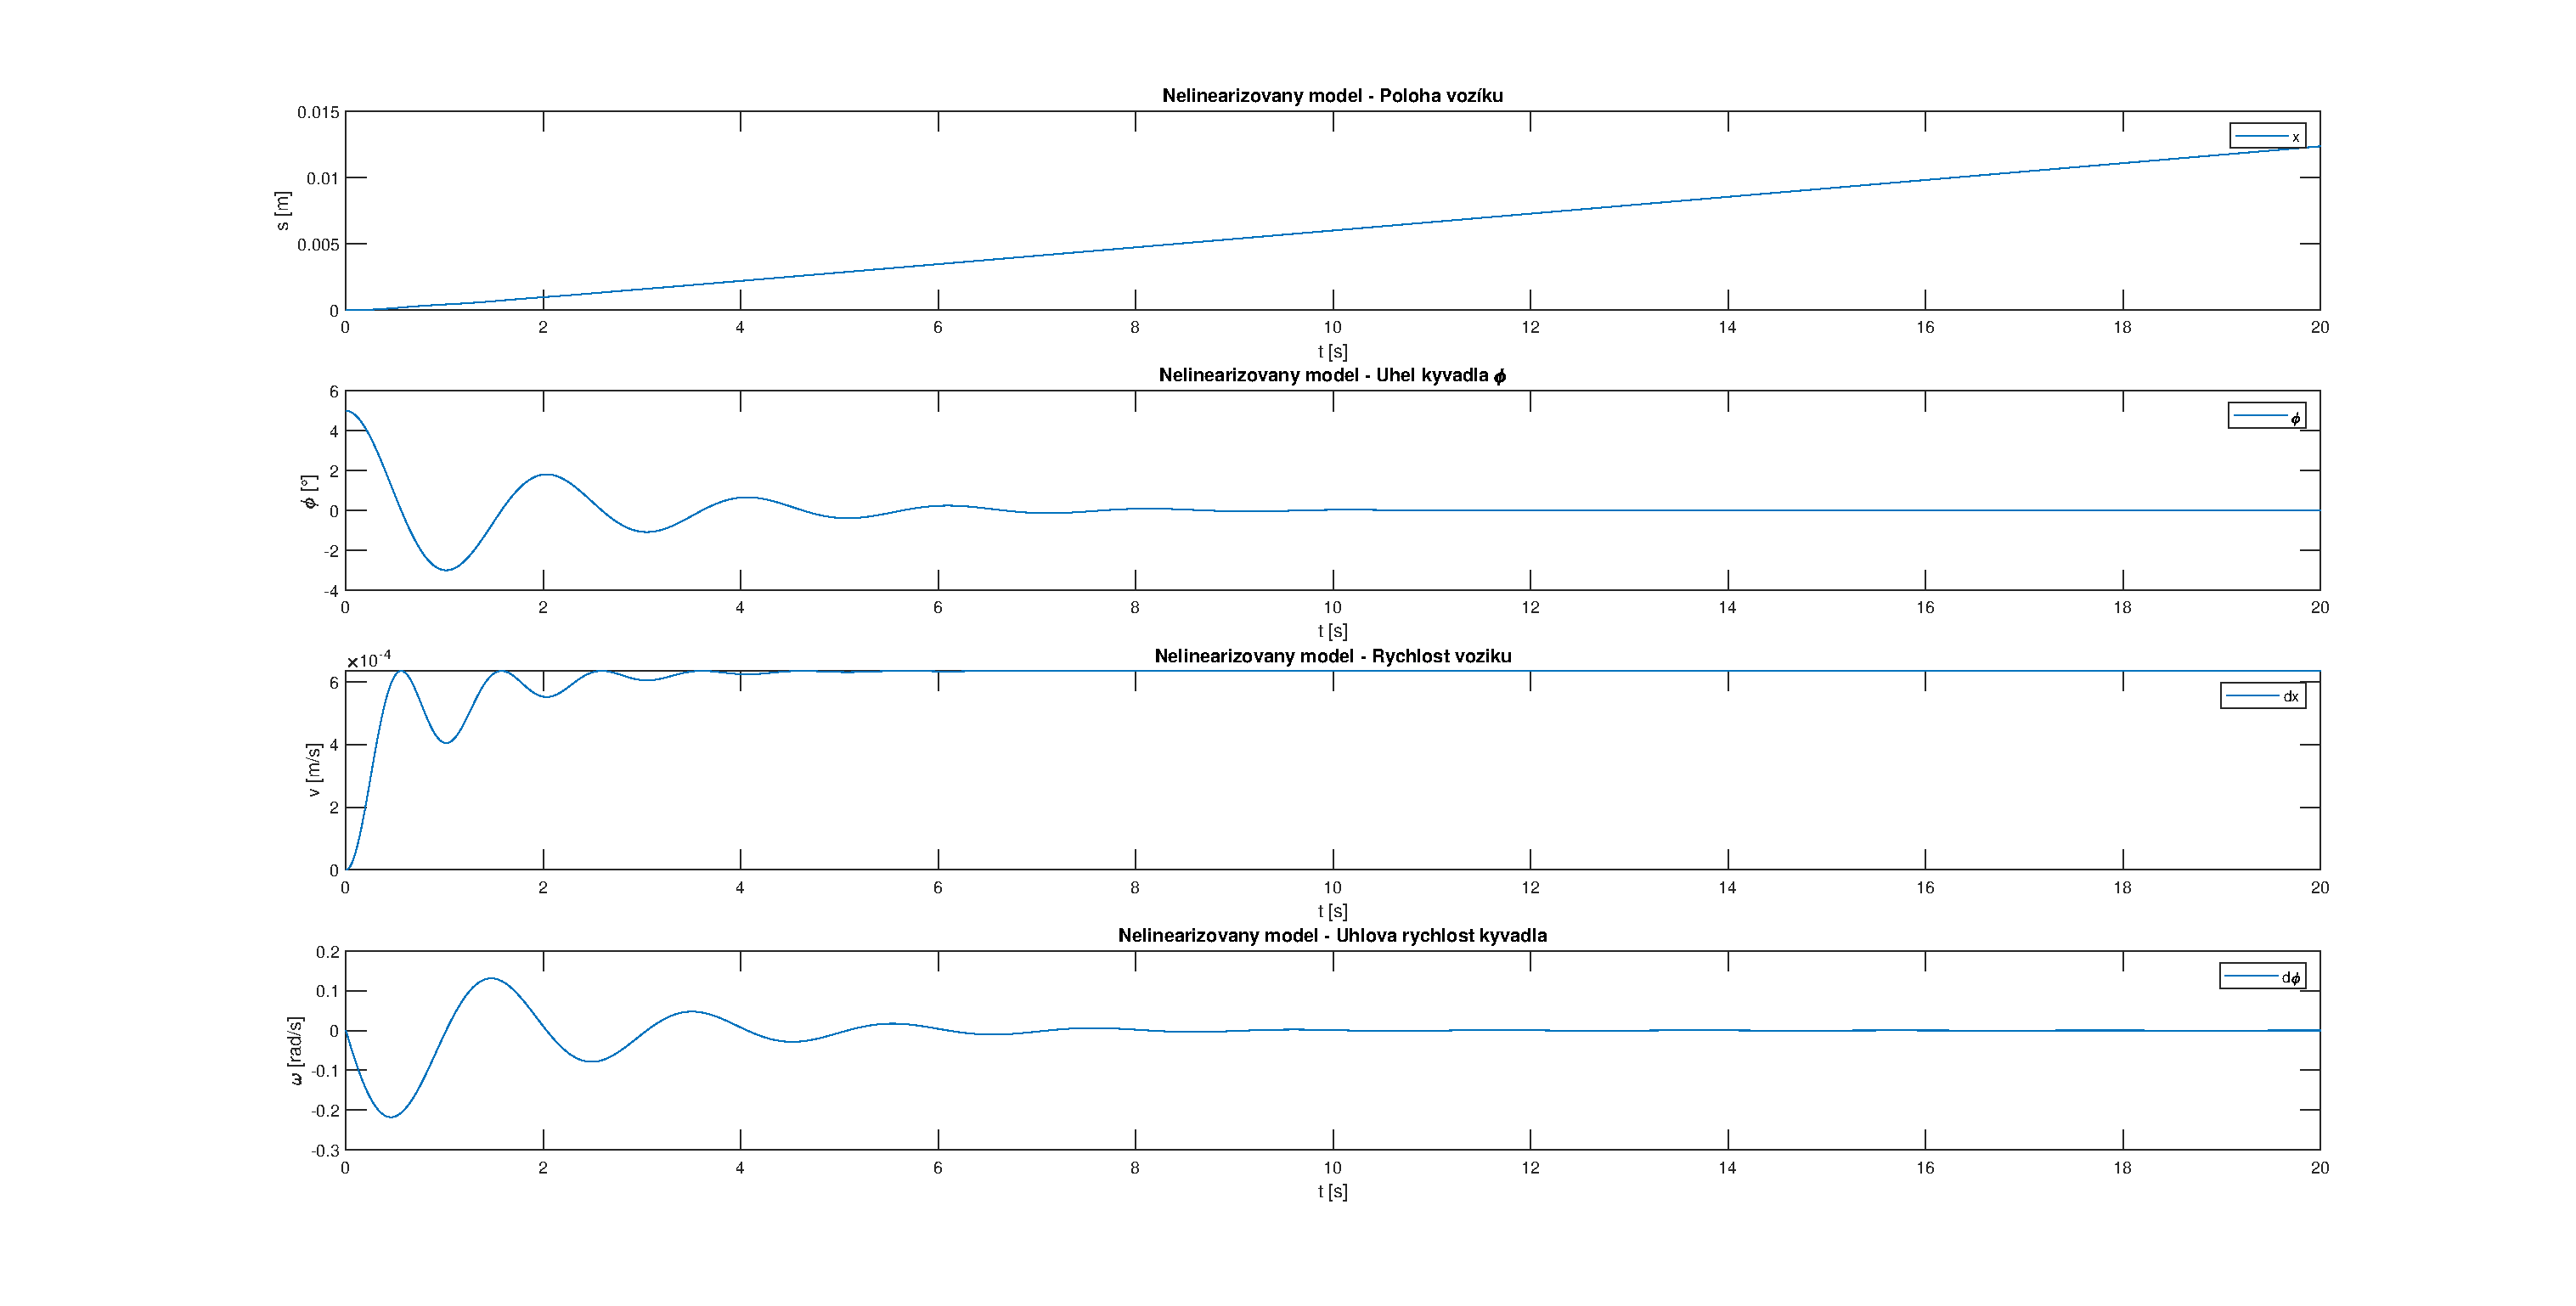
\includegraphics[scale=0.33]{Obrazky/Nelin_model_f0_nenul.eps}
					\label{Nel_model_f0_nenul}
					\caption{Nelineární model při $f=\SI{0}{\newton}$ a p.p. $\varphi = \SI{5}{\degree}$}
				\end{center}
				\begin{center}
					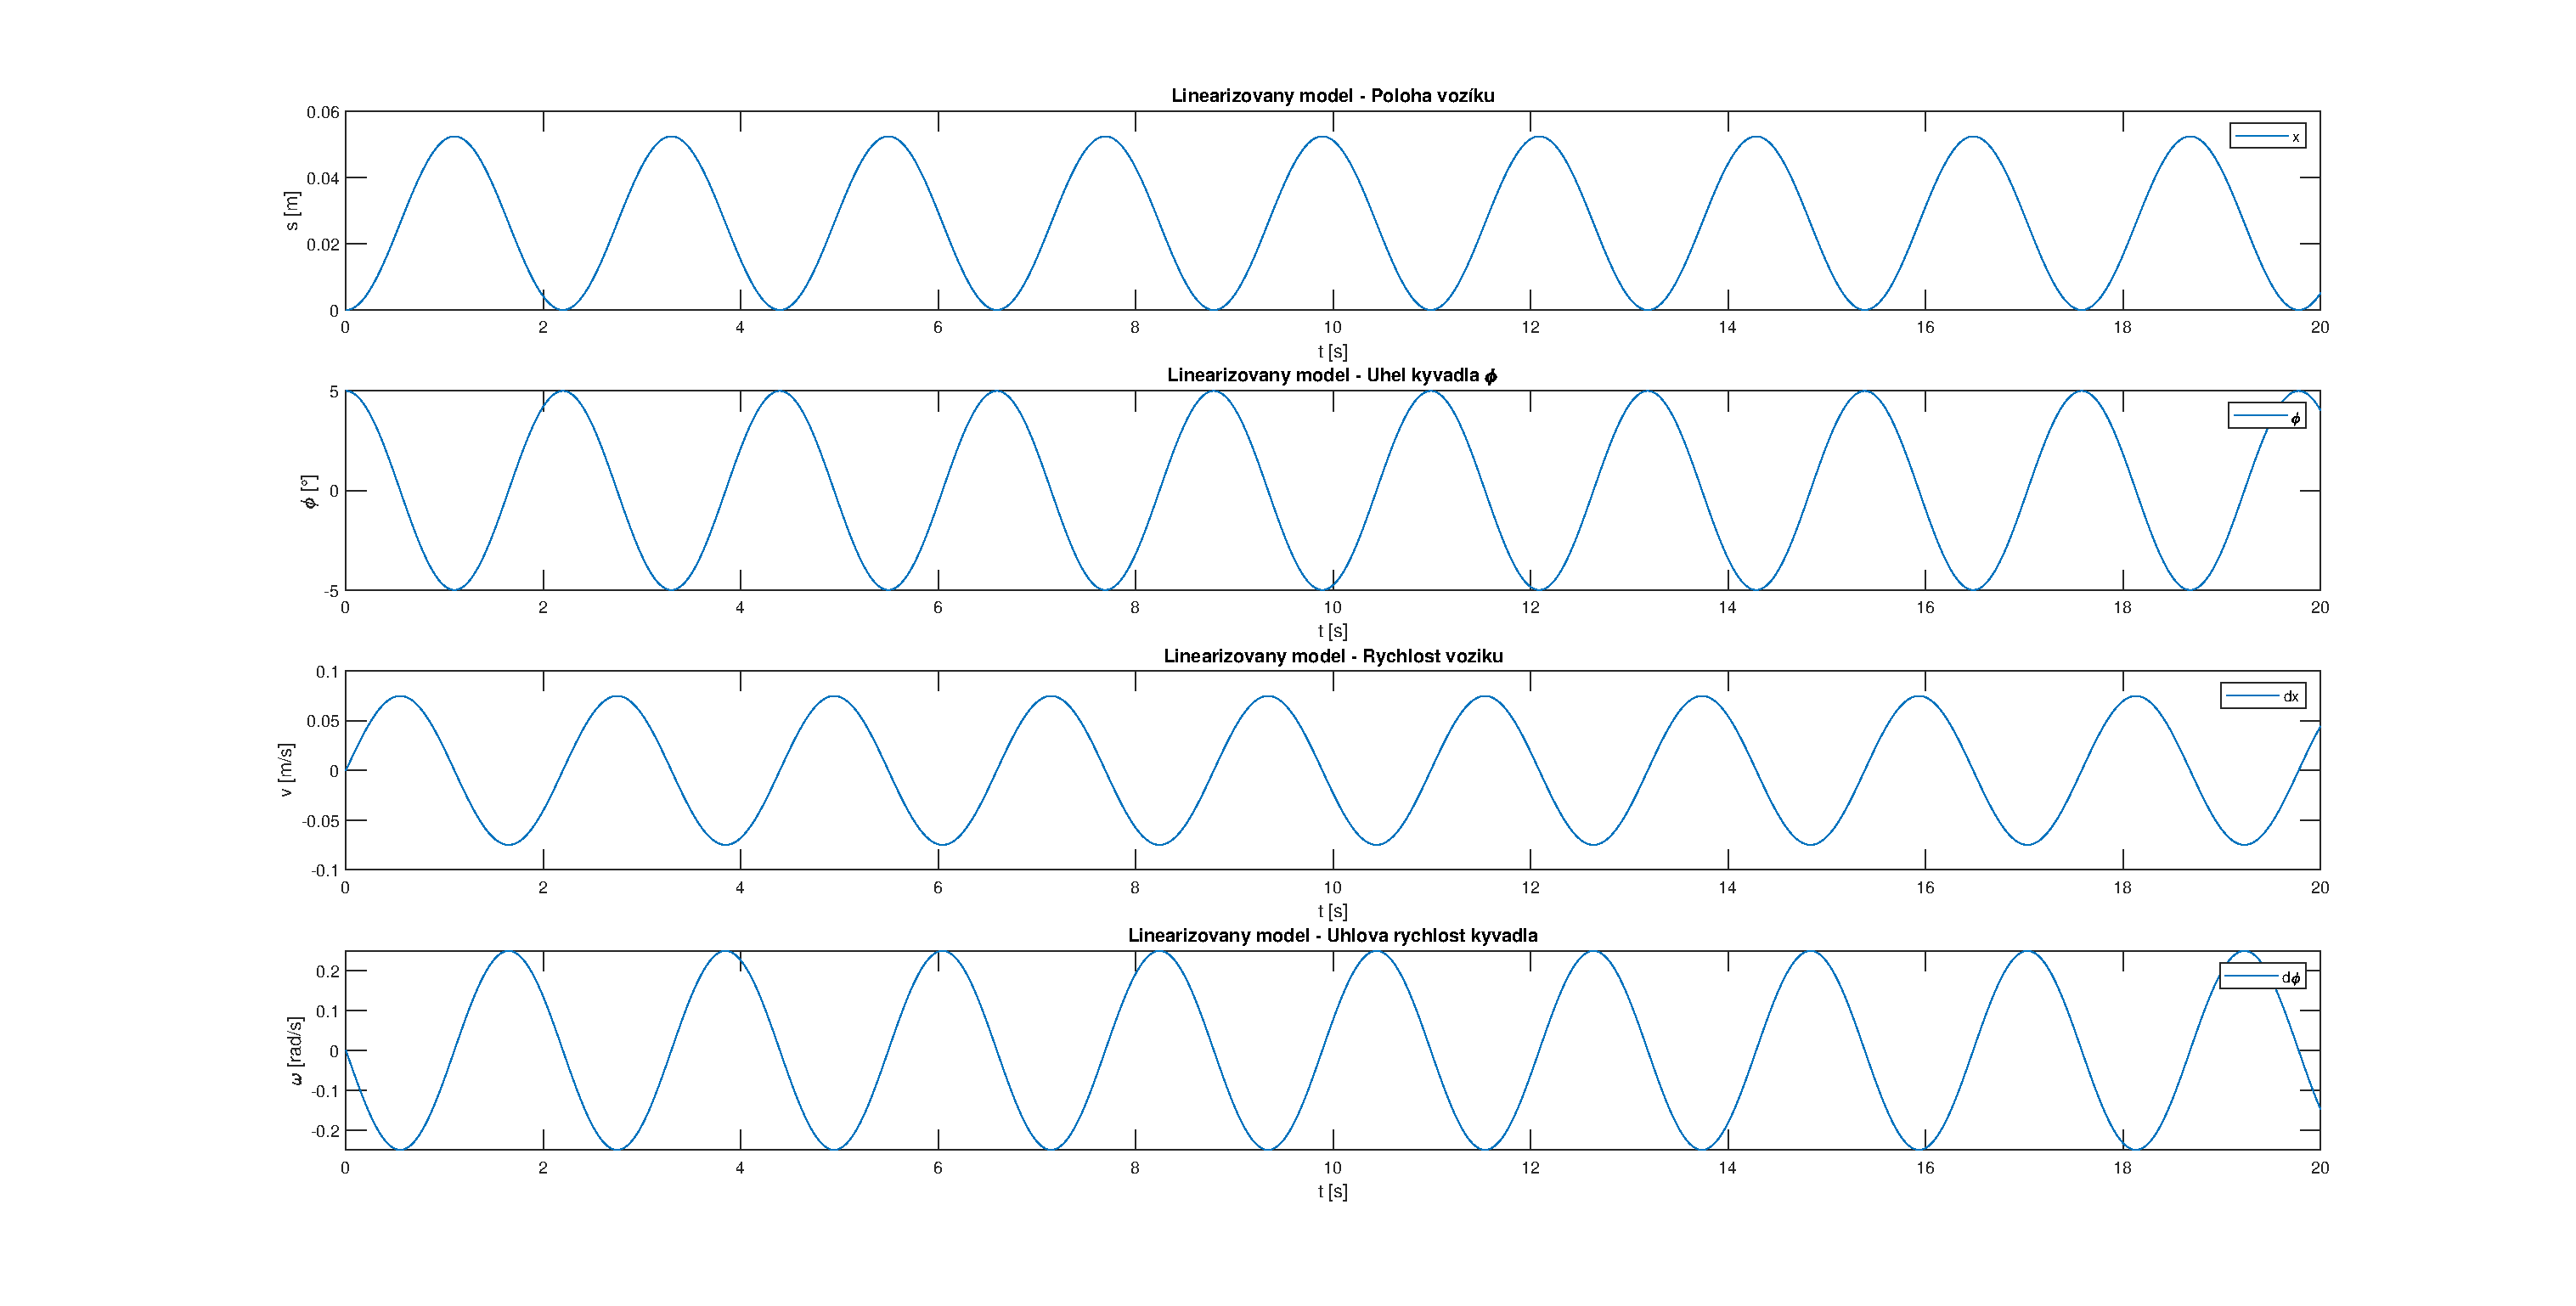
\includegraphics[scale=0.33]{Obrazky/Lin_model_f0_nenul.eps}
					\label{Lin_model_f0_nenul}
					\caption{Lineární model při $f=\SI{0}{\newton}$ a p.p. $\varphi = \SI{5}{\degree}$}
				\end{center}
			\end{figure}
			\begin{figure}[h]
				\begin{center}
					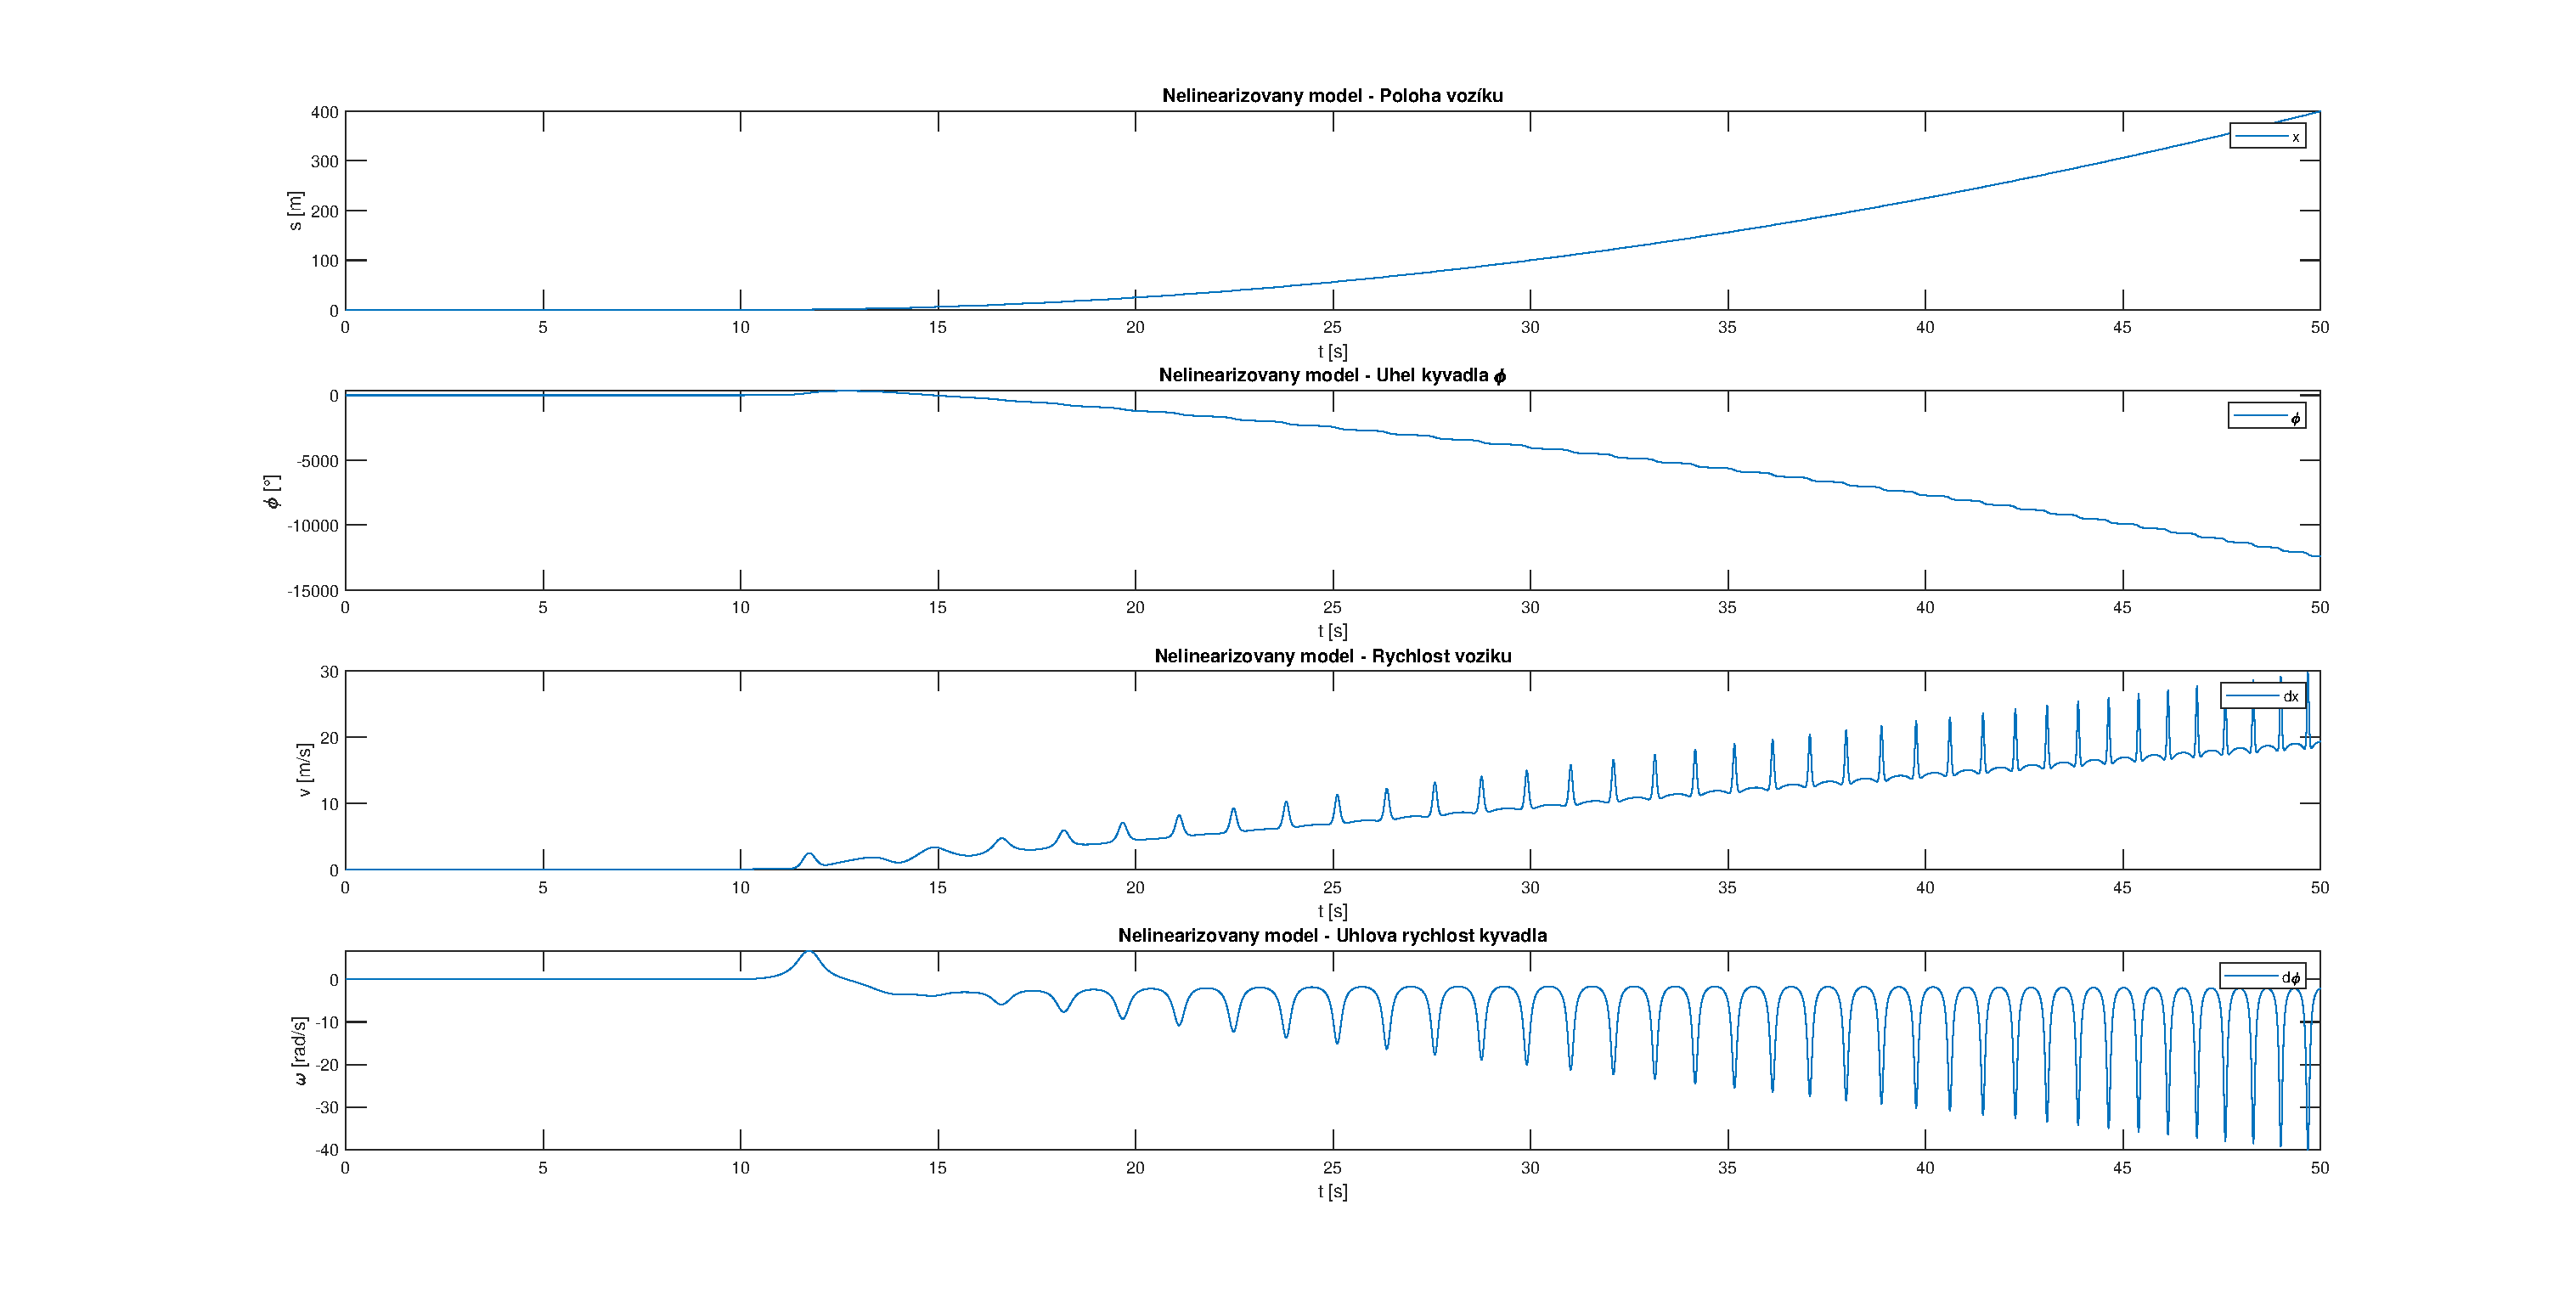
\includegraphics[scale=0.33]{Obrazky/Nel_model_f10_nul.eps}
					\label{Nel_model_f10_nul}
					\caption{Nelineární model při $f=\SI{10}{\newton}$ a nulových p.p.}
				\end{center}
				\begin{center}
					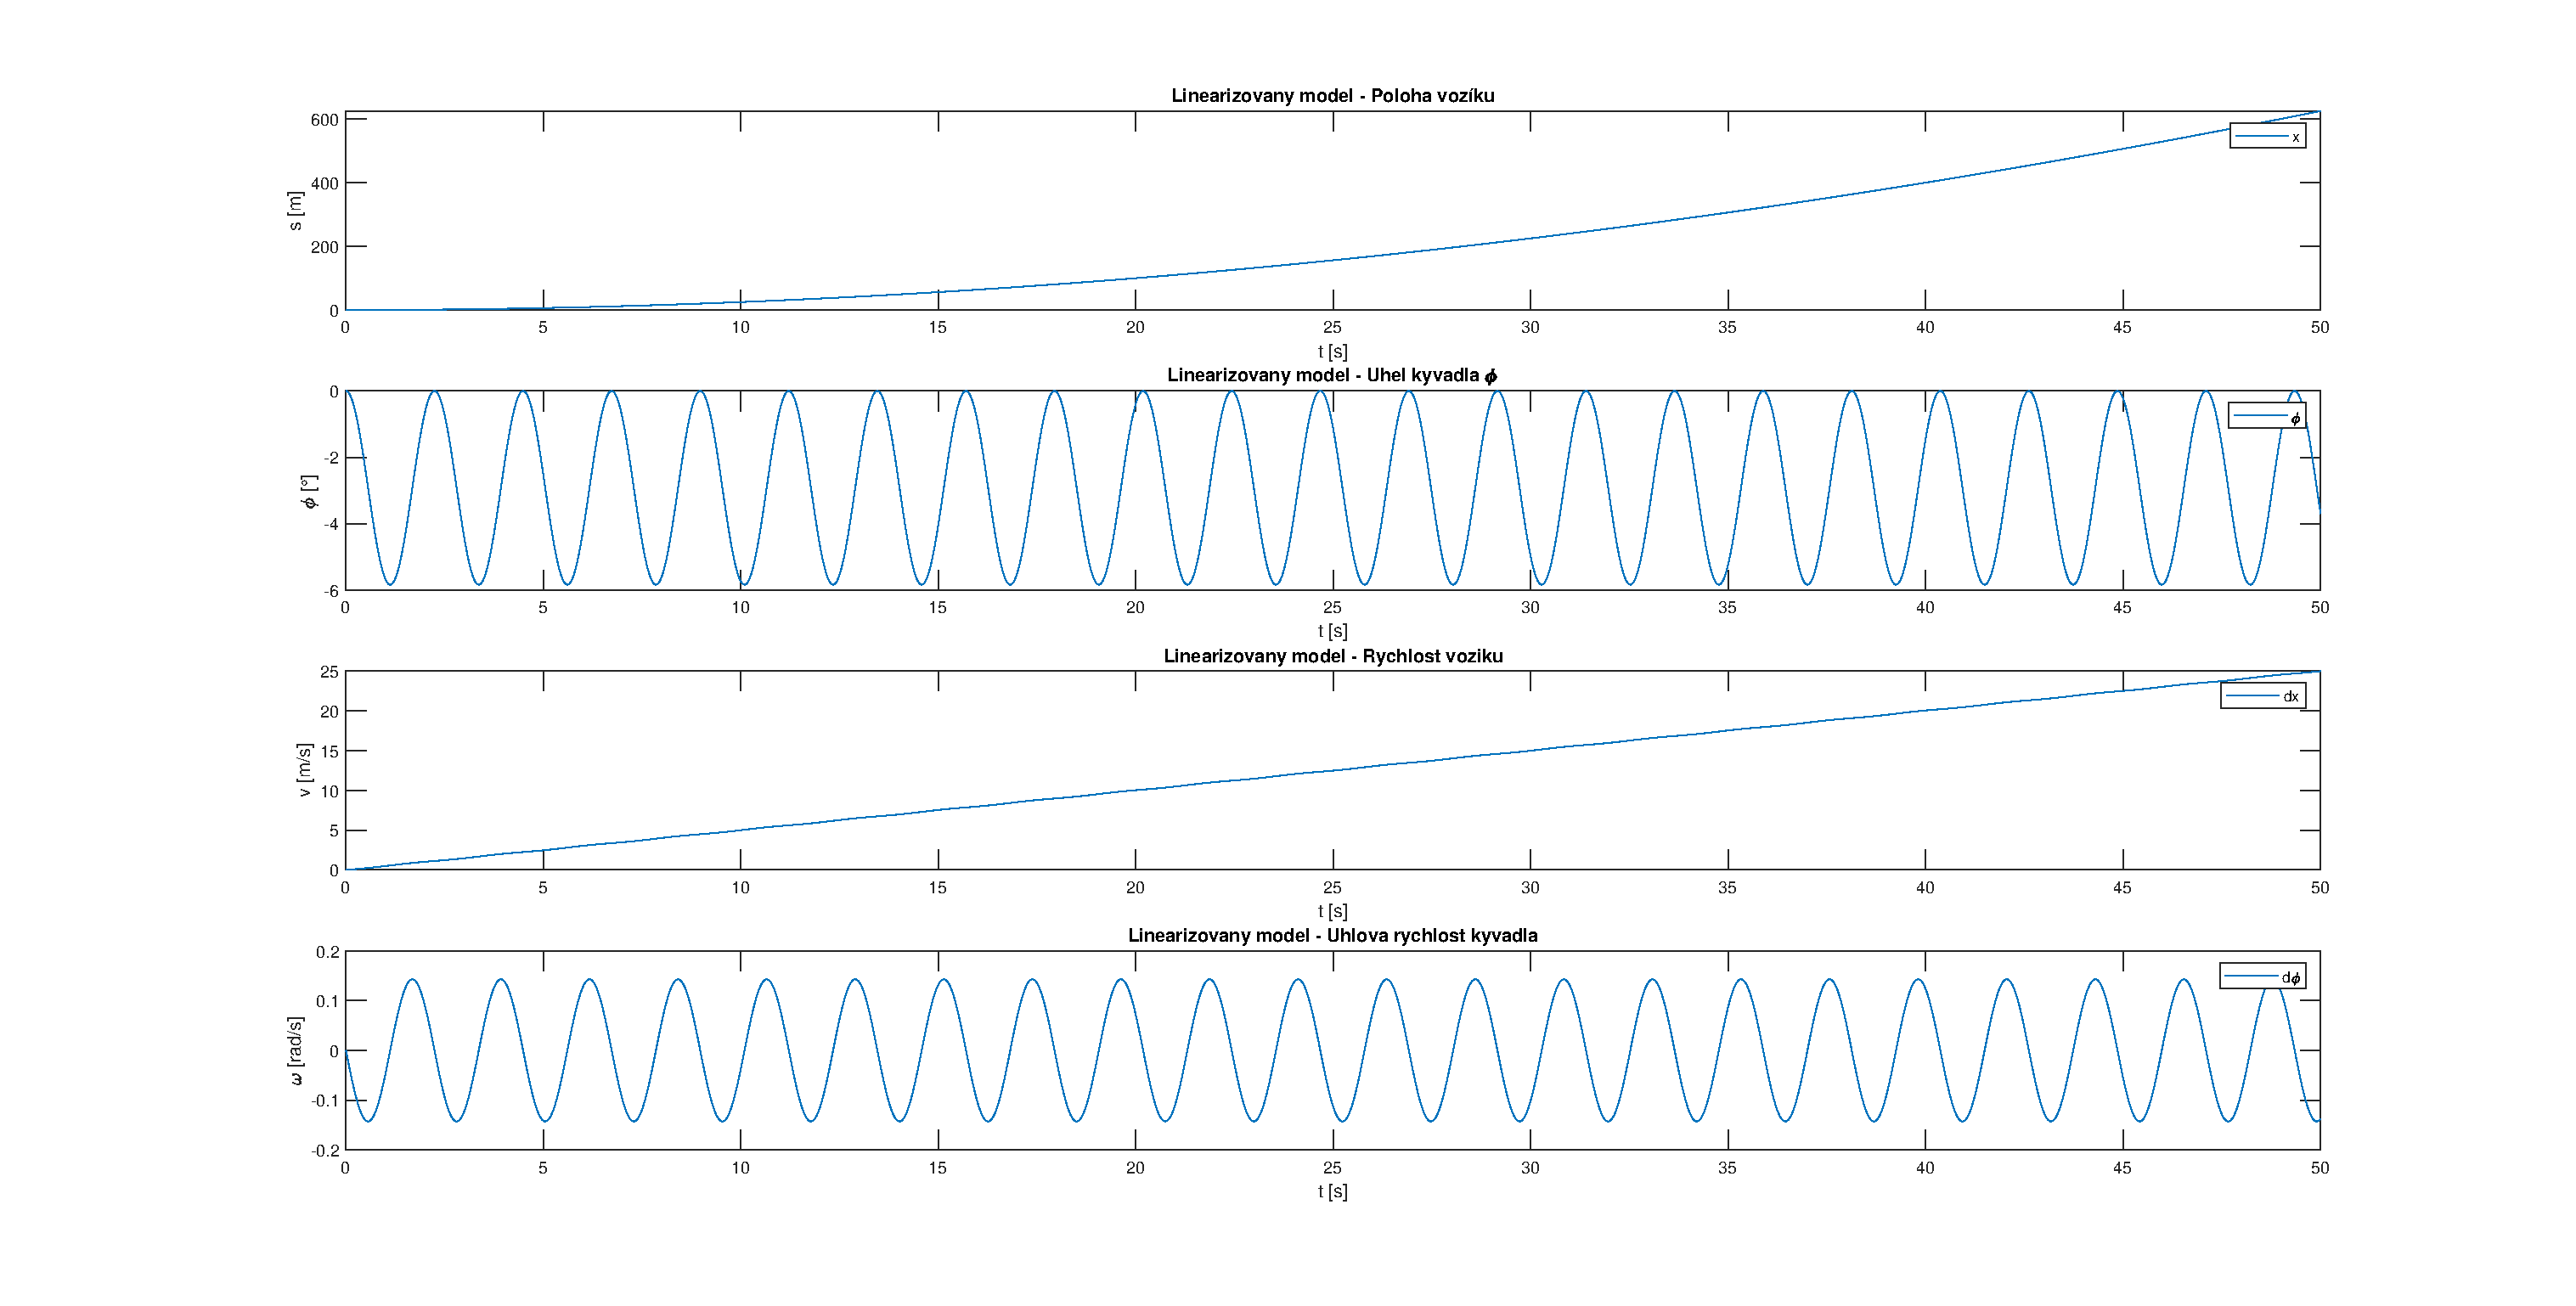
\includegraphics[scale=0.33]{Obrazky/Lin_model_f10_nul.eps}
					\label{Lin_model_f10_nul}
					\caption{Lineární model při $f=\SI{10}{\newton}$ a nulových p.p.}
				\end{center}
			\end{figure}
			\begin{figure}[h]
				\begin{center}
					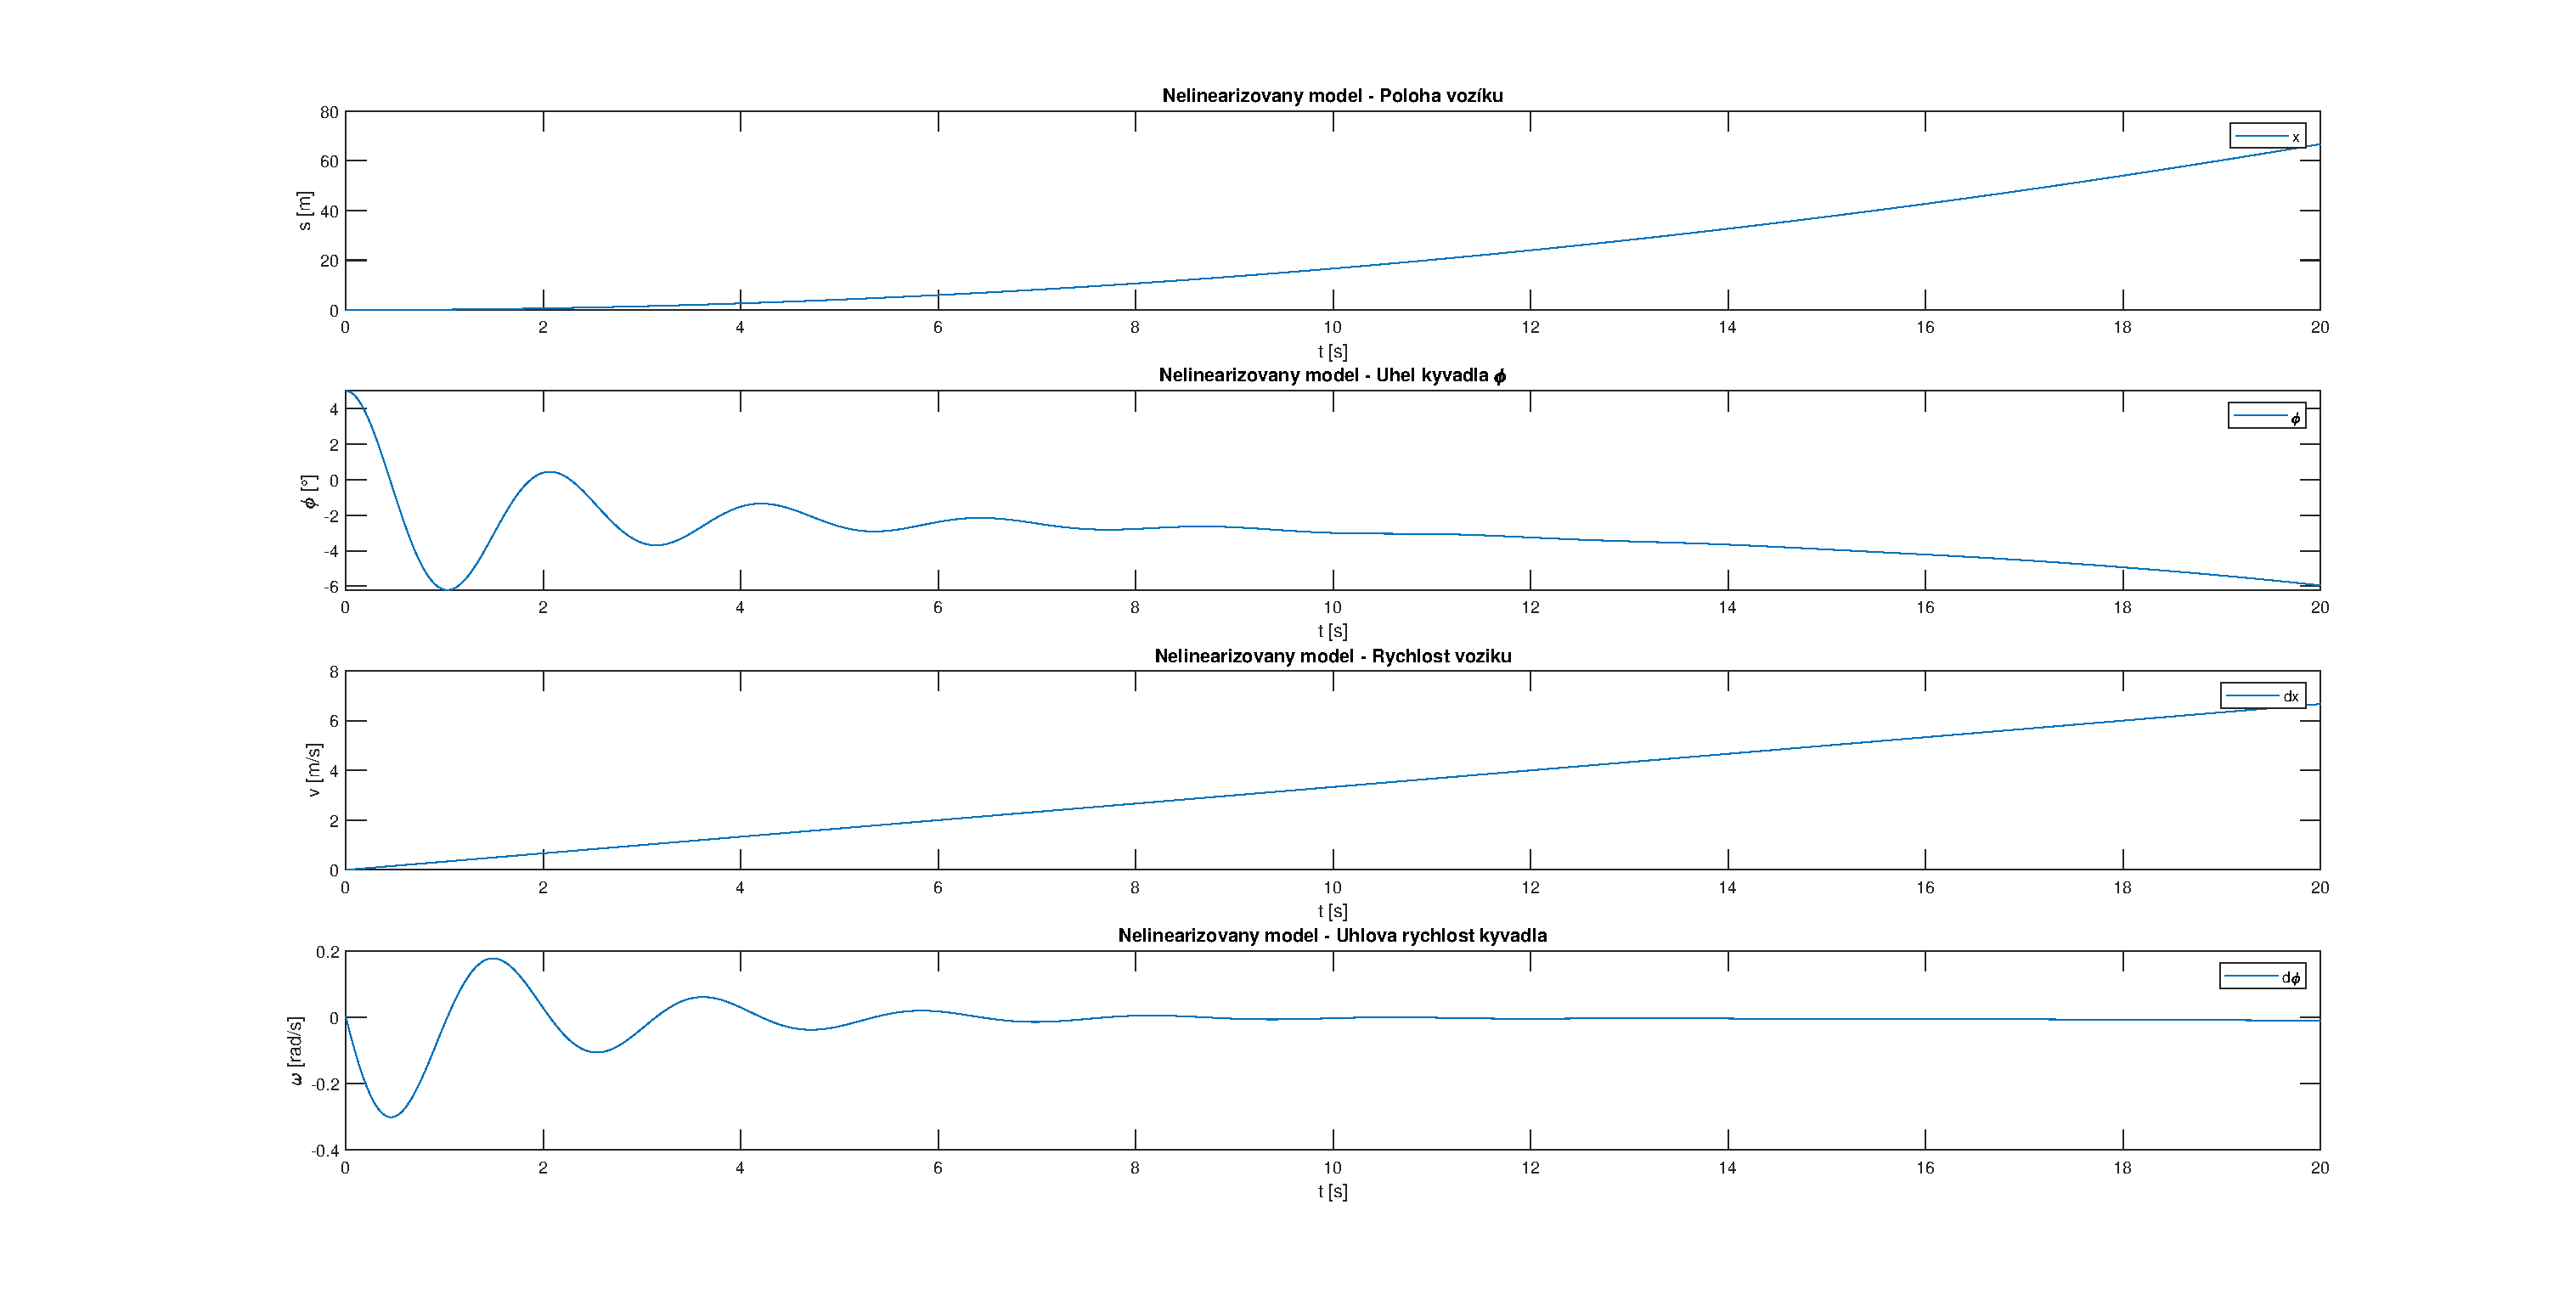
\includegraphics[scale=0.33]{Obrazky/Nel_model_f10_nenul.eps}
					\label{Nel_model_f10_nenul}
					\caption{Nelineární model při $f=\SI{10}{\newton}$ a p.p. $\varphi = \SI{5}{\degree}$}
				\end{center}
				\begin{center}
					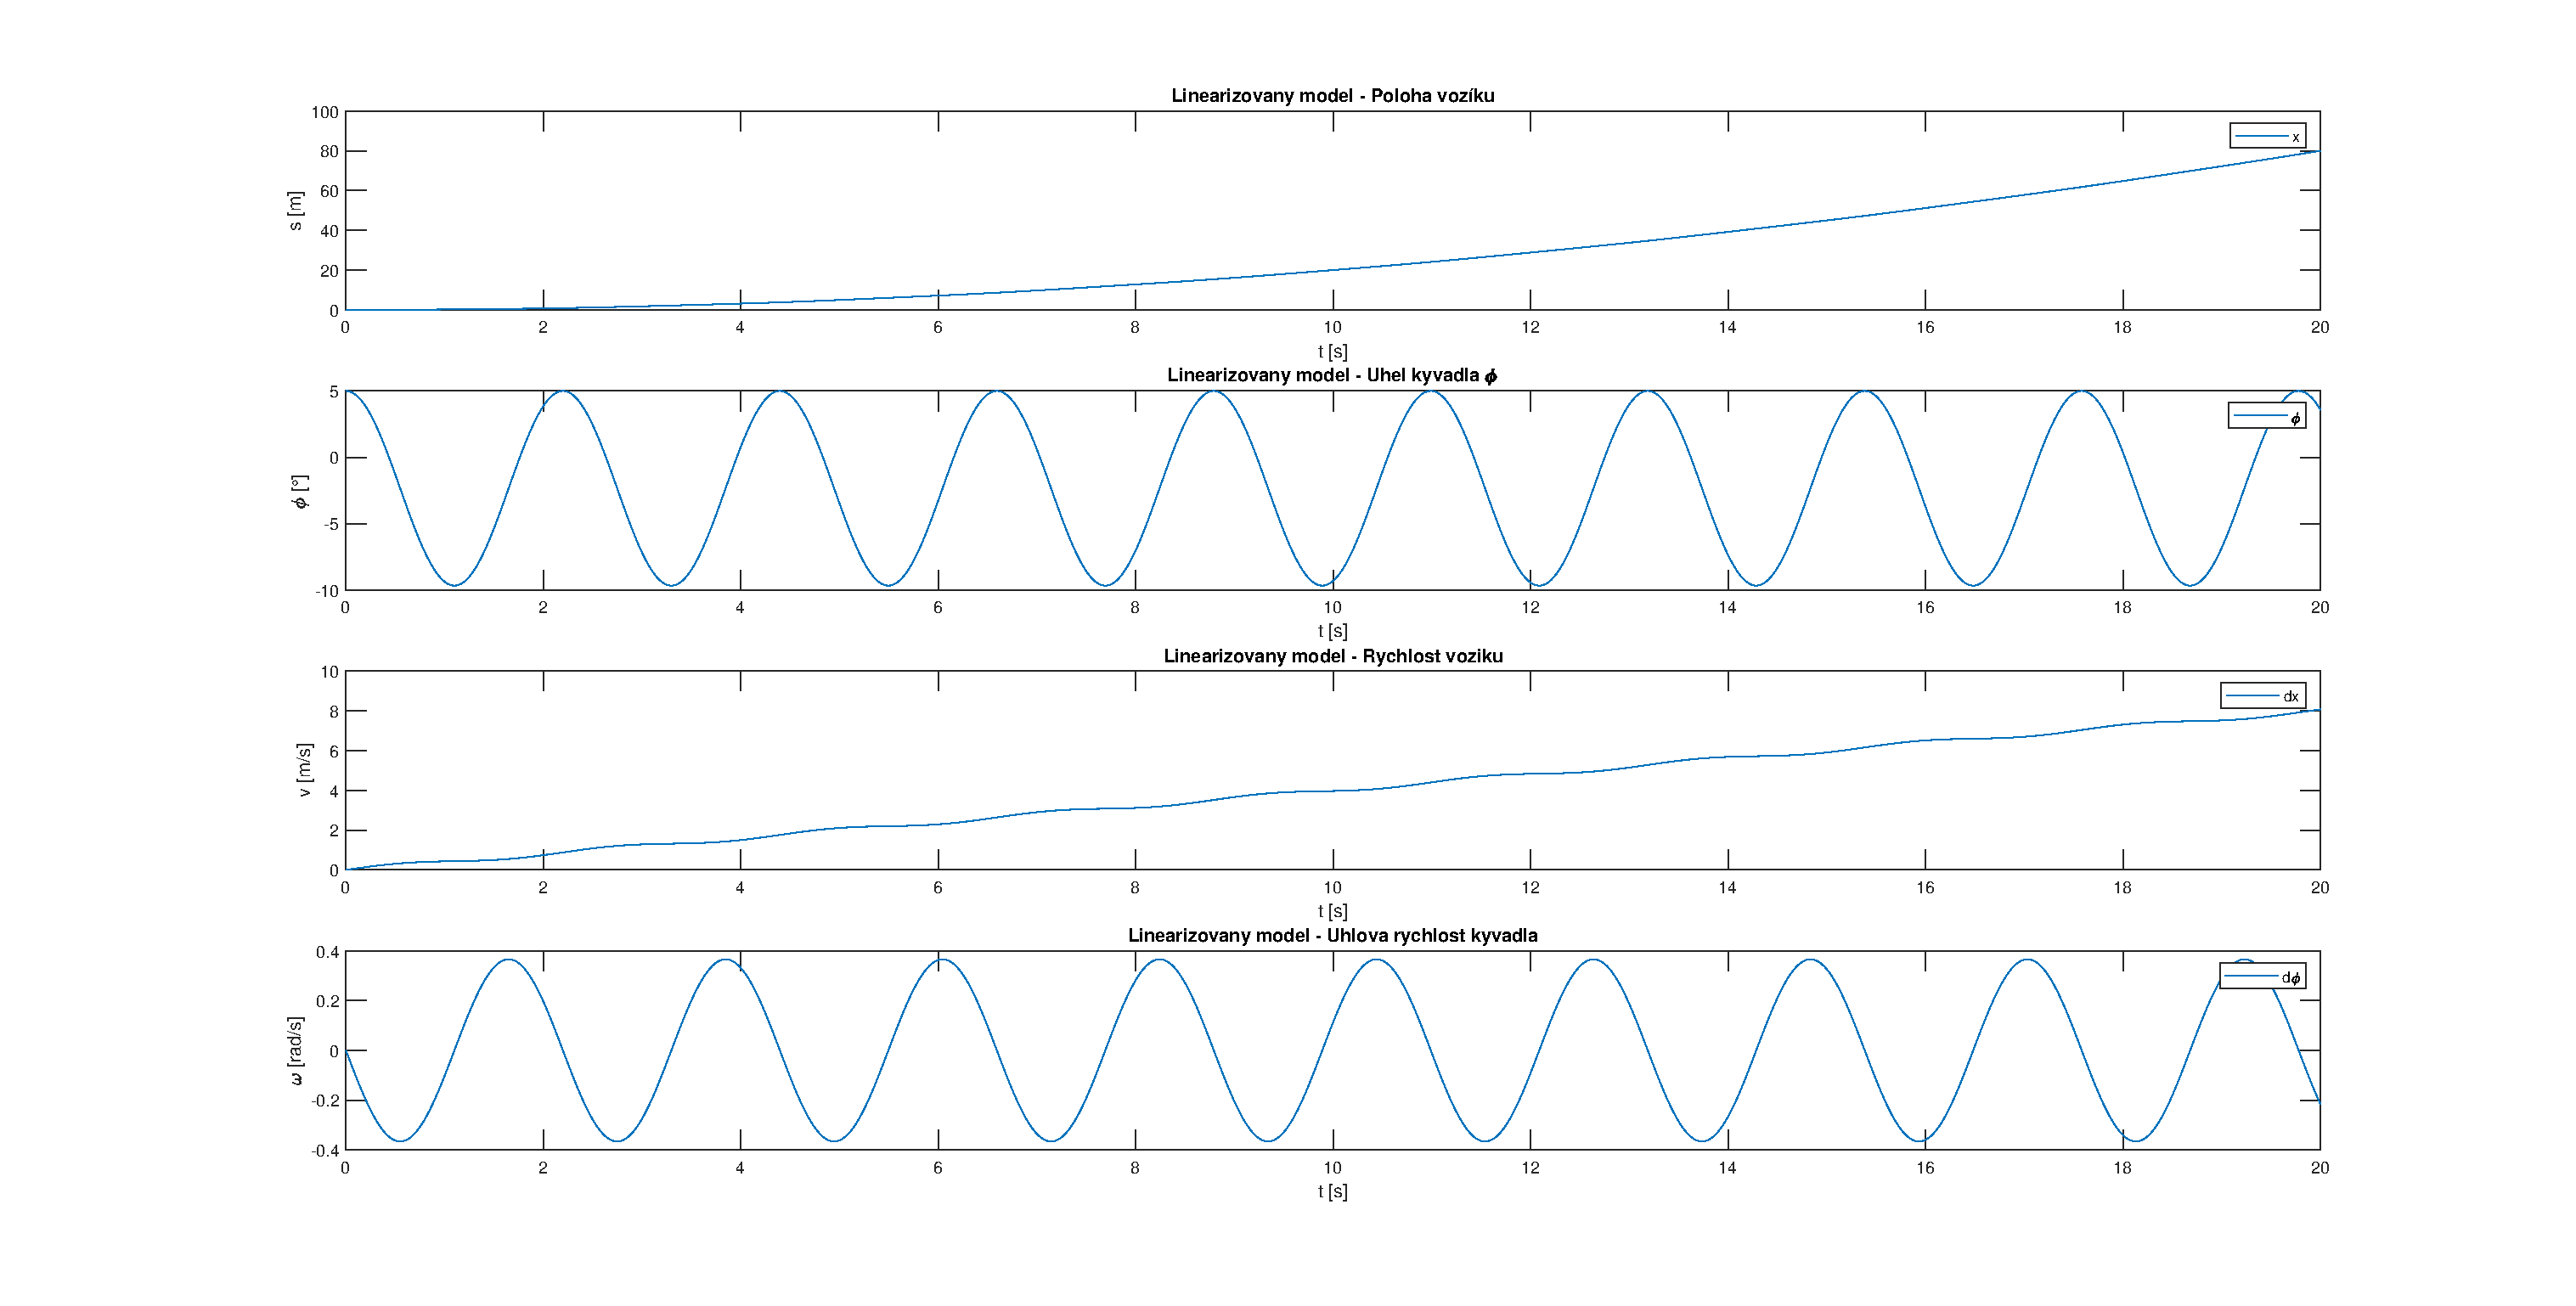
\includegraphics[scale=0.33]{Obrazky/Lin_model_f10_nenul.eps}
					\label{Lin_model_f10_nenul}
					\caption{Lineární model při $f=\SI{10}{\newton}$ a p.p. $\varphi = \SI{5}{\degree}$}
				\end{center}
			\end{figure}
	\clearpage
	\section{Návrh regulátoru}
		Jako nejideálnější regulátor jsme zvolili regulátor stavový. Cílem bylo ustabilizovat systém, tzn. dostat póly systému na mezi stability (obr. \ref{GMK_na_mezi}) do záporné poloroviny a tím systém učinit stabilním.	
		\begin{figure}[h]
			\begin{center}
				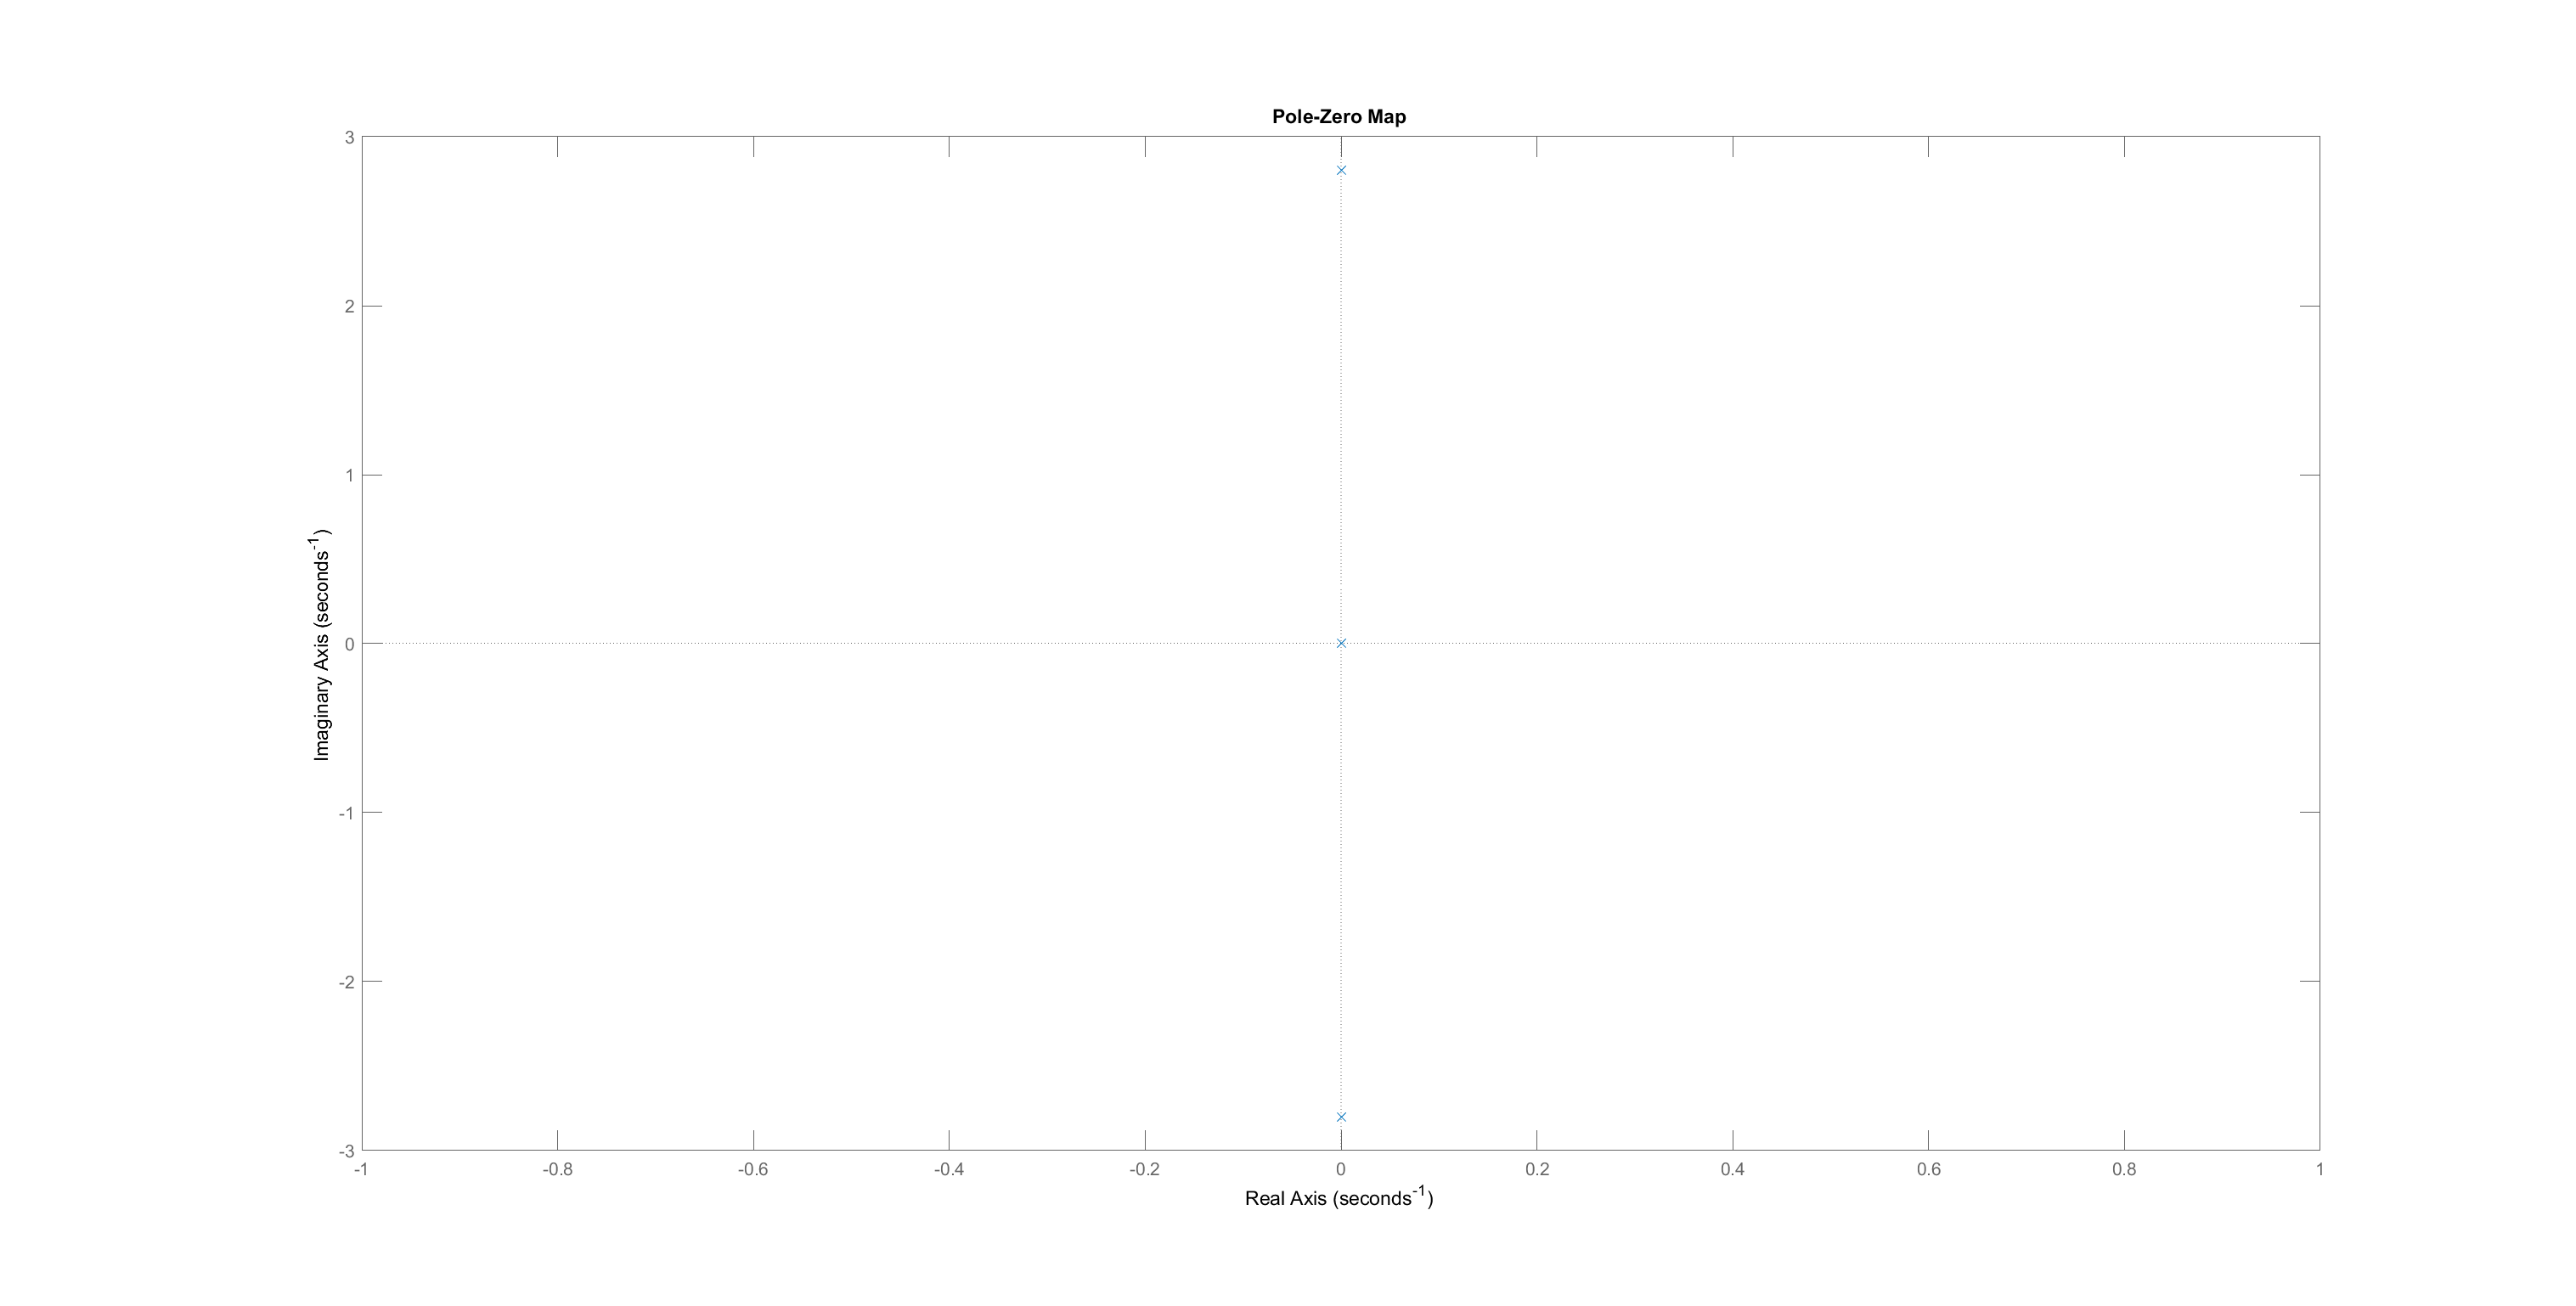
\includegraphics[scale=0.33]{Obrazky/GMK_na_mezi.eps}
				\label{GMK_na_mezi}
				\caption{GMK systému na mezi stability}
			\end{center}
		\end{figure}
		\\Nejprve je potřeba si zvolit požadované póly. V našem případě máme čtyři póly s nulovou reálnou částí (to způsobuje kmitání systému, který je díky tomu na mezi stability). Musíme tak zvolit póly, které mají zápornou reálnou část. Nyní můžeme vypočítat vektor zesílení $K$. Toho dosáhneme např. v Matlabu pomocí funkce $\texttt{K = acker(A, B, p)}$, kde \texttt{A} je matice systému, \texttt{B} je matice řízení a \texttt{p} je vektor požadovaných pólů. Po získání vektoru zesílení je možno vytvořit uzavřenou zpětnou vazbu systému ve stavovém popisu podle vzorce:
		\begin{align*}
			A_u &= A-B*K\\
			B_u &= B\\
			C_u &= C\\
			D_u &= D
		\end{align*}
		\\Můžeme tedy vyzkoušet, jak se bude nově vzniklý systém chovat při nulových počátečních podmínkách (obr. \ref{Stav_reg_f0_nul}) a nenulových počátečních podmínkách (obr. \ref{Stav_reg_f0_nenul}).
		\begin{figure}[h]
			\begin{center}
				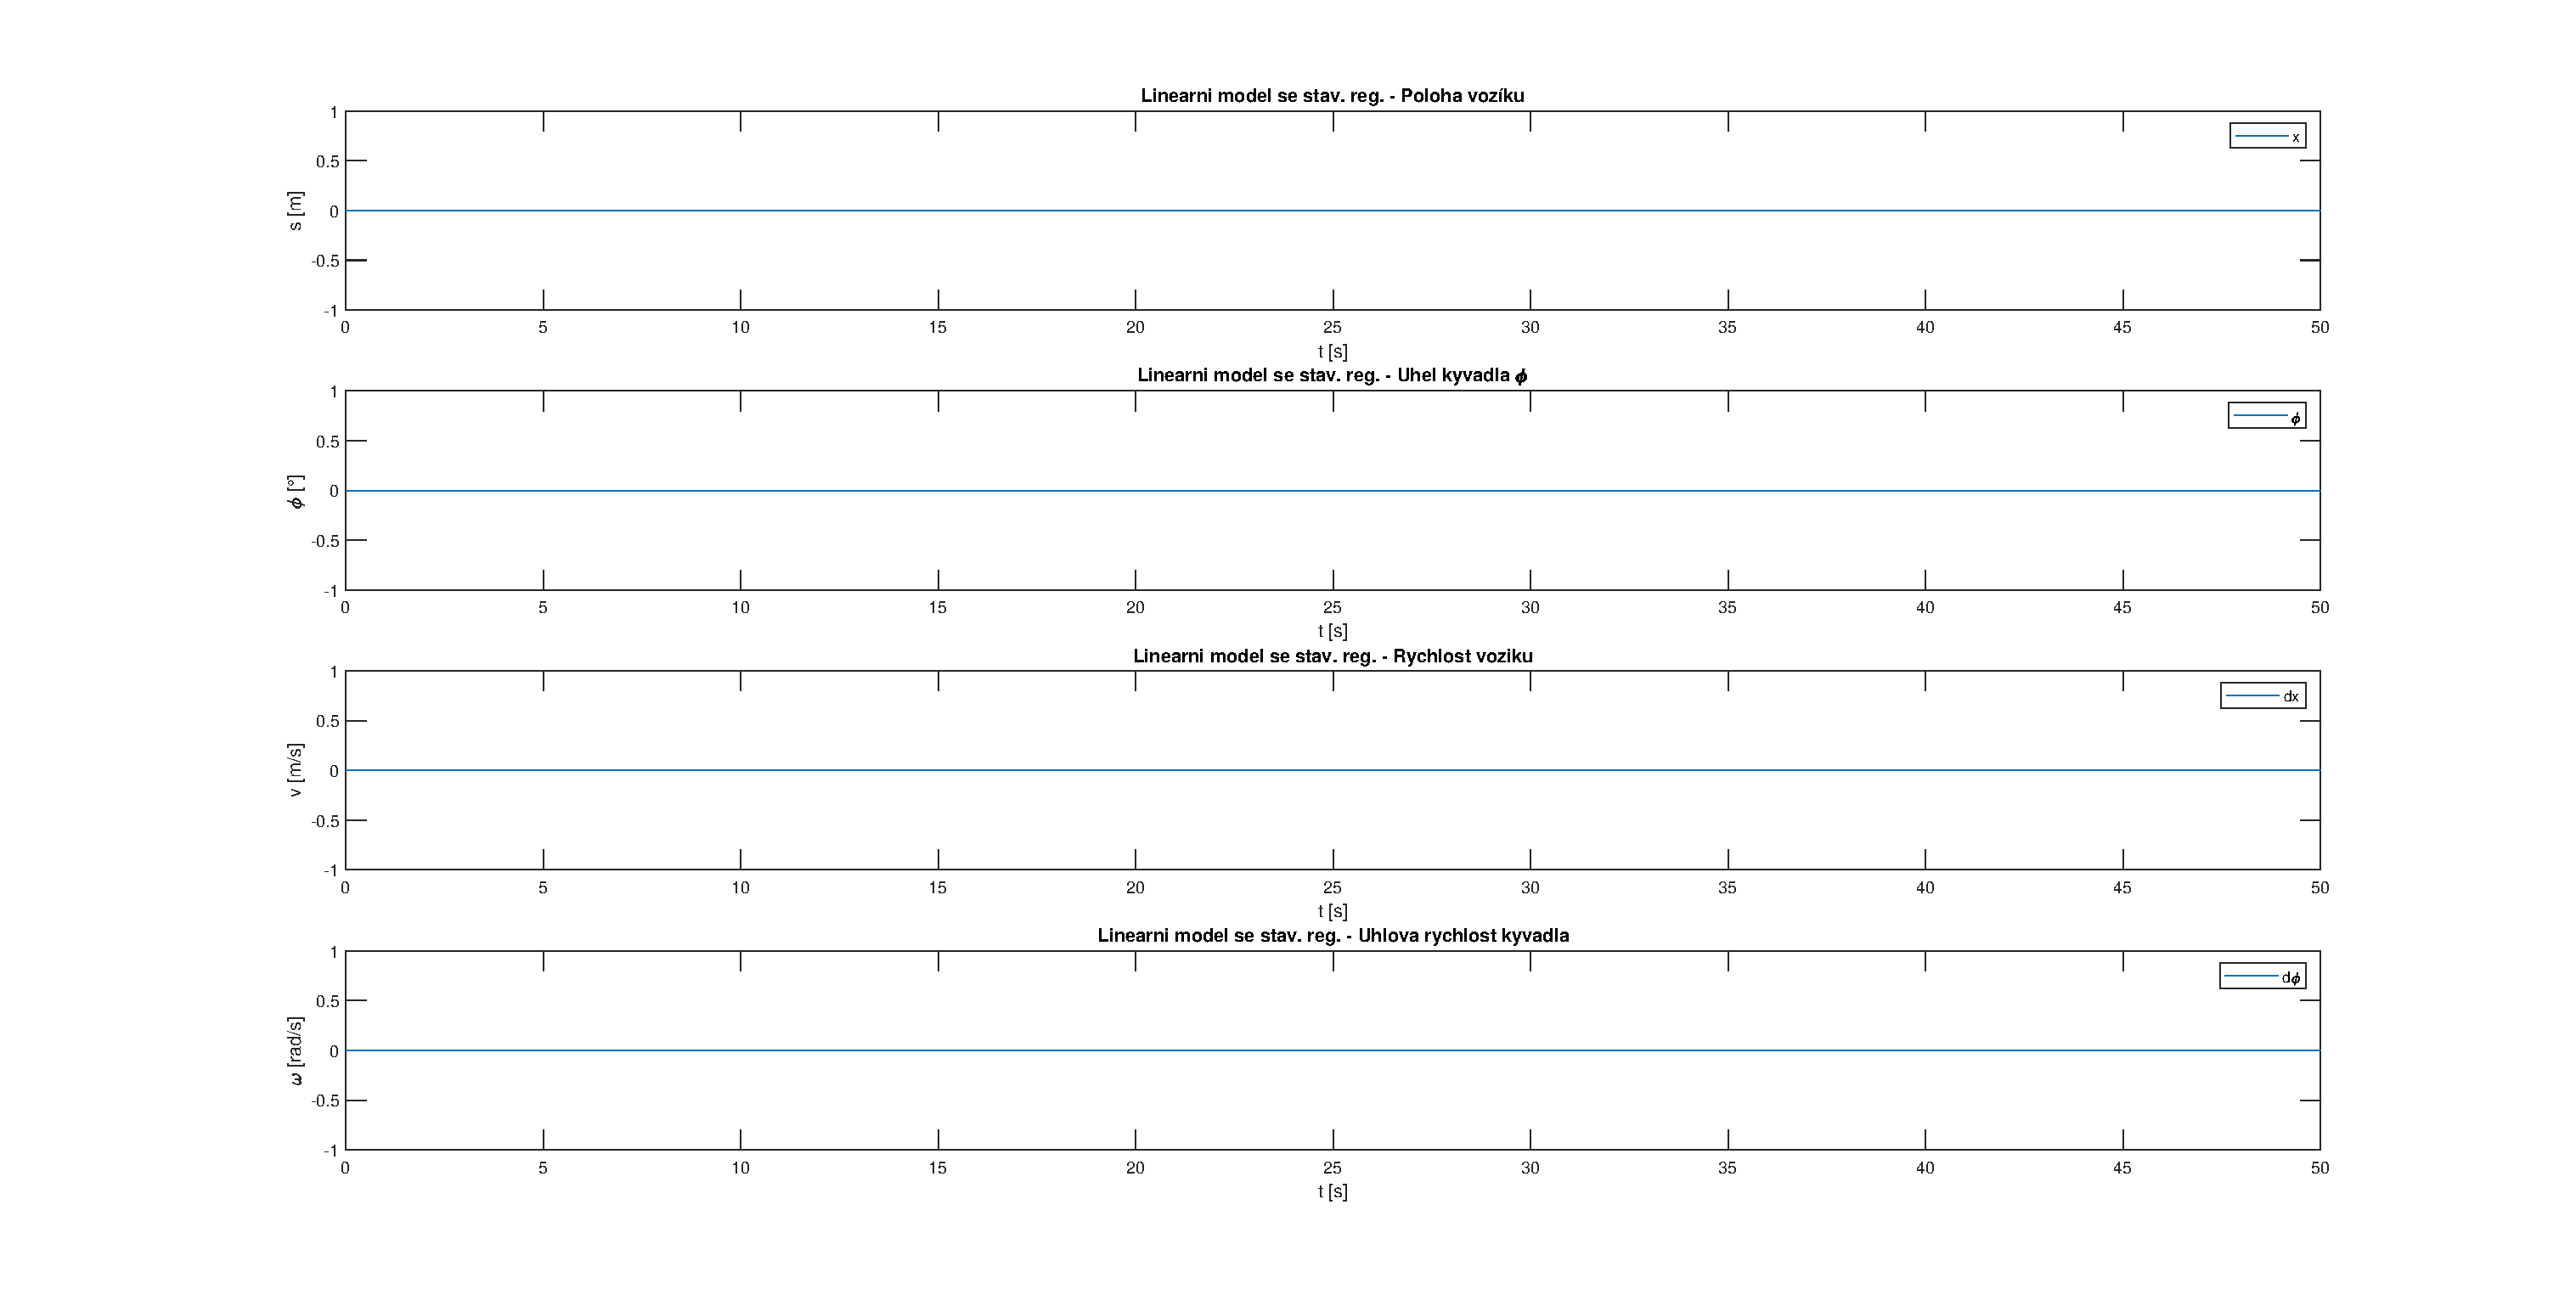
\includegraphics[scale=0.33]{Obrazky/Stav_reg_f0_nul.eps}
				\label{Stav_reg_f0_nul}
				\caption{Lineární model se stav. reg. při p.p. $\varphi = \SI{0}{\degree}$}
			\end{center}
			\begin{center}
				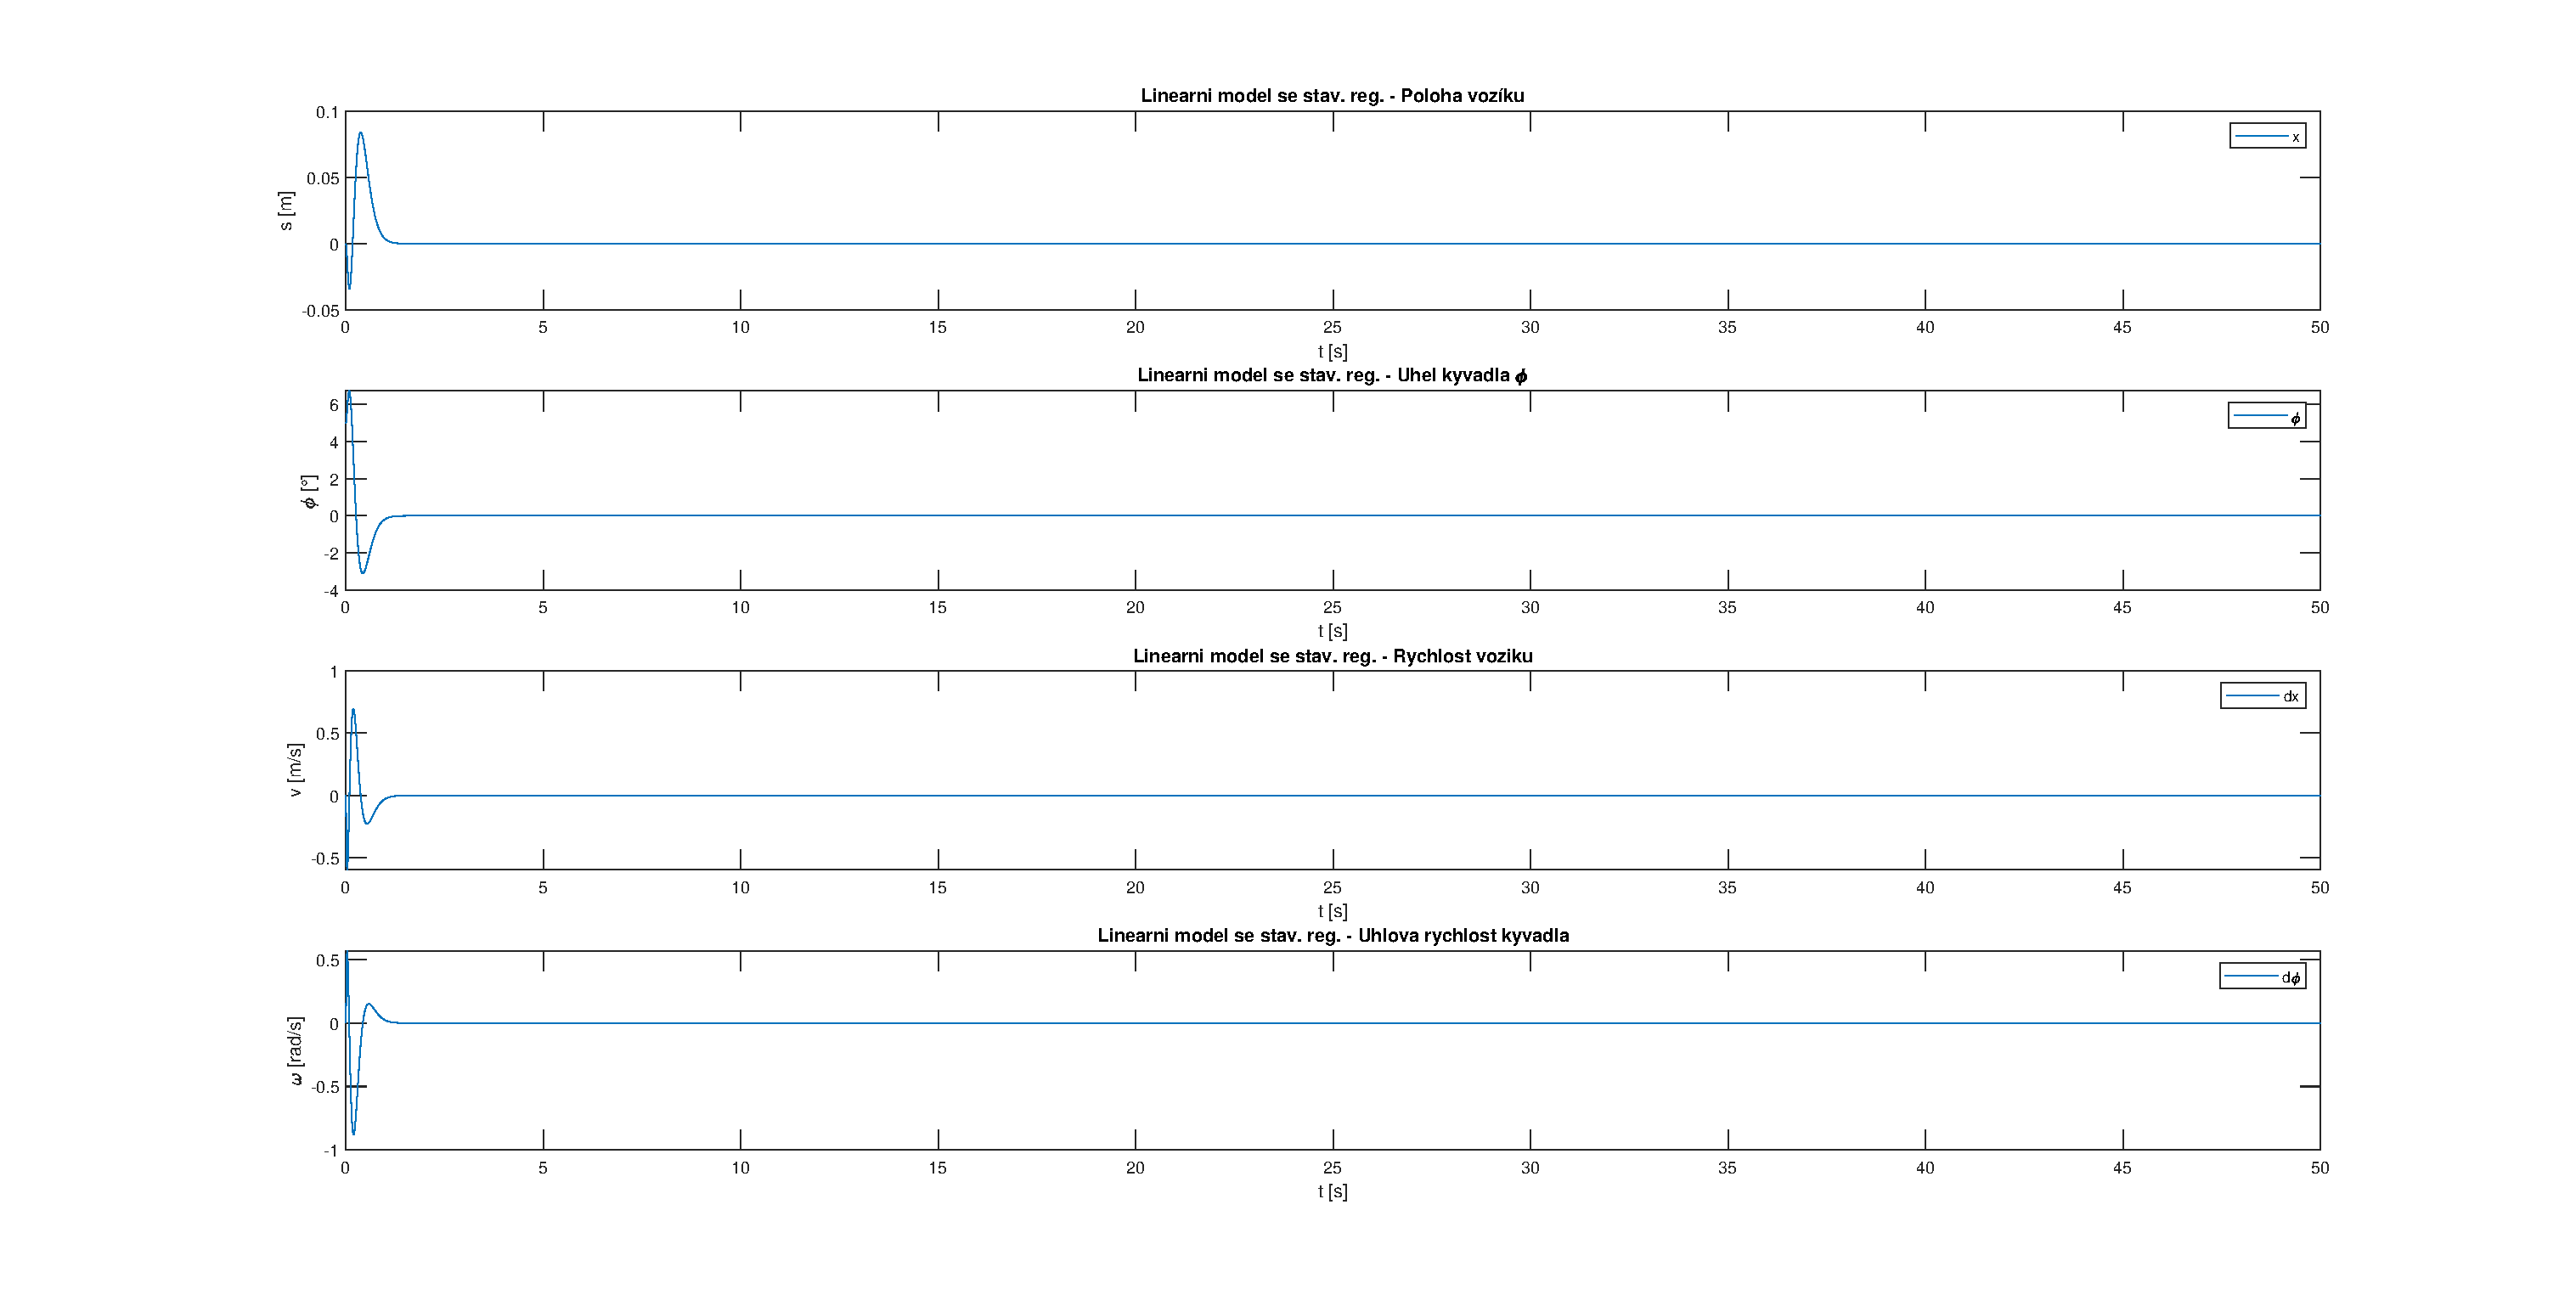
\includegraphics[scale=0.33]{Obrazky/Stav_reg_f0_nenul.eps}
				\label{Stav_reg_f0_nenul}
				\caption{Lineární model se stav. reg. při p.p. $\varphi = \SI{0}{\degree}$}
			\end{center}
		\end{figure}
		\\Z obou obrázků je vidět, že systém je stabilní.
		
\end{document}